\section{Introduction}

\msb{A note for the eventual TOCHI paper on HabitLab: it's generally frowned upon to use large sections of your own prior text. Check out TOCHI or CHI's self-plagiarism policy, think about what might need to be expanded or rewritten for a TOCHI paper. It's fine in a thesis.}

\msb{For now or for TOCHI: this chapter will need to articulate more forcefully what the contribution of the tool is. What's novel about it?}

Studying behavior change requires in-the-wild intervention and observation~\cite{consolvo2008activity}. Inspired by previous CSCW tools for naturalistic data collection~\cite{reinecke2015labinthewild}, we developed HabitLab~\cite{habitlab}, an open-source\footnote{HabitLab is available at \url{http://habitlab.github.io}.} platform, as a living laboratory to help us understand online behavior change and as a platform to explore novel behavior change designs (Figure~\ref{fig:homepage}).

% HabitLab is a Chrome browser extension and Android application that contains a variety of productivity interventions. It aims to help users reduce their time spent online on web pages that the user specifies (e.g., Facebook, Twitter, and Reddit). The system is pitched to end users as a tool that explores various different interventions (referred to as ``nudges'') to help them reduce their time on sites.

HabitLab is a Chrome browser extension and Android application that contains a variety of productivity interventions. It aims to help users reduce their time spent online on web pages that the user specifies (e.g., Facebook, Twitter, and Reddit). The system is pitched to end users as a tool that explores various different interventions (referred to as ``nudges'') to help them reduce their time on sites.


\begin{figure}
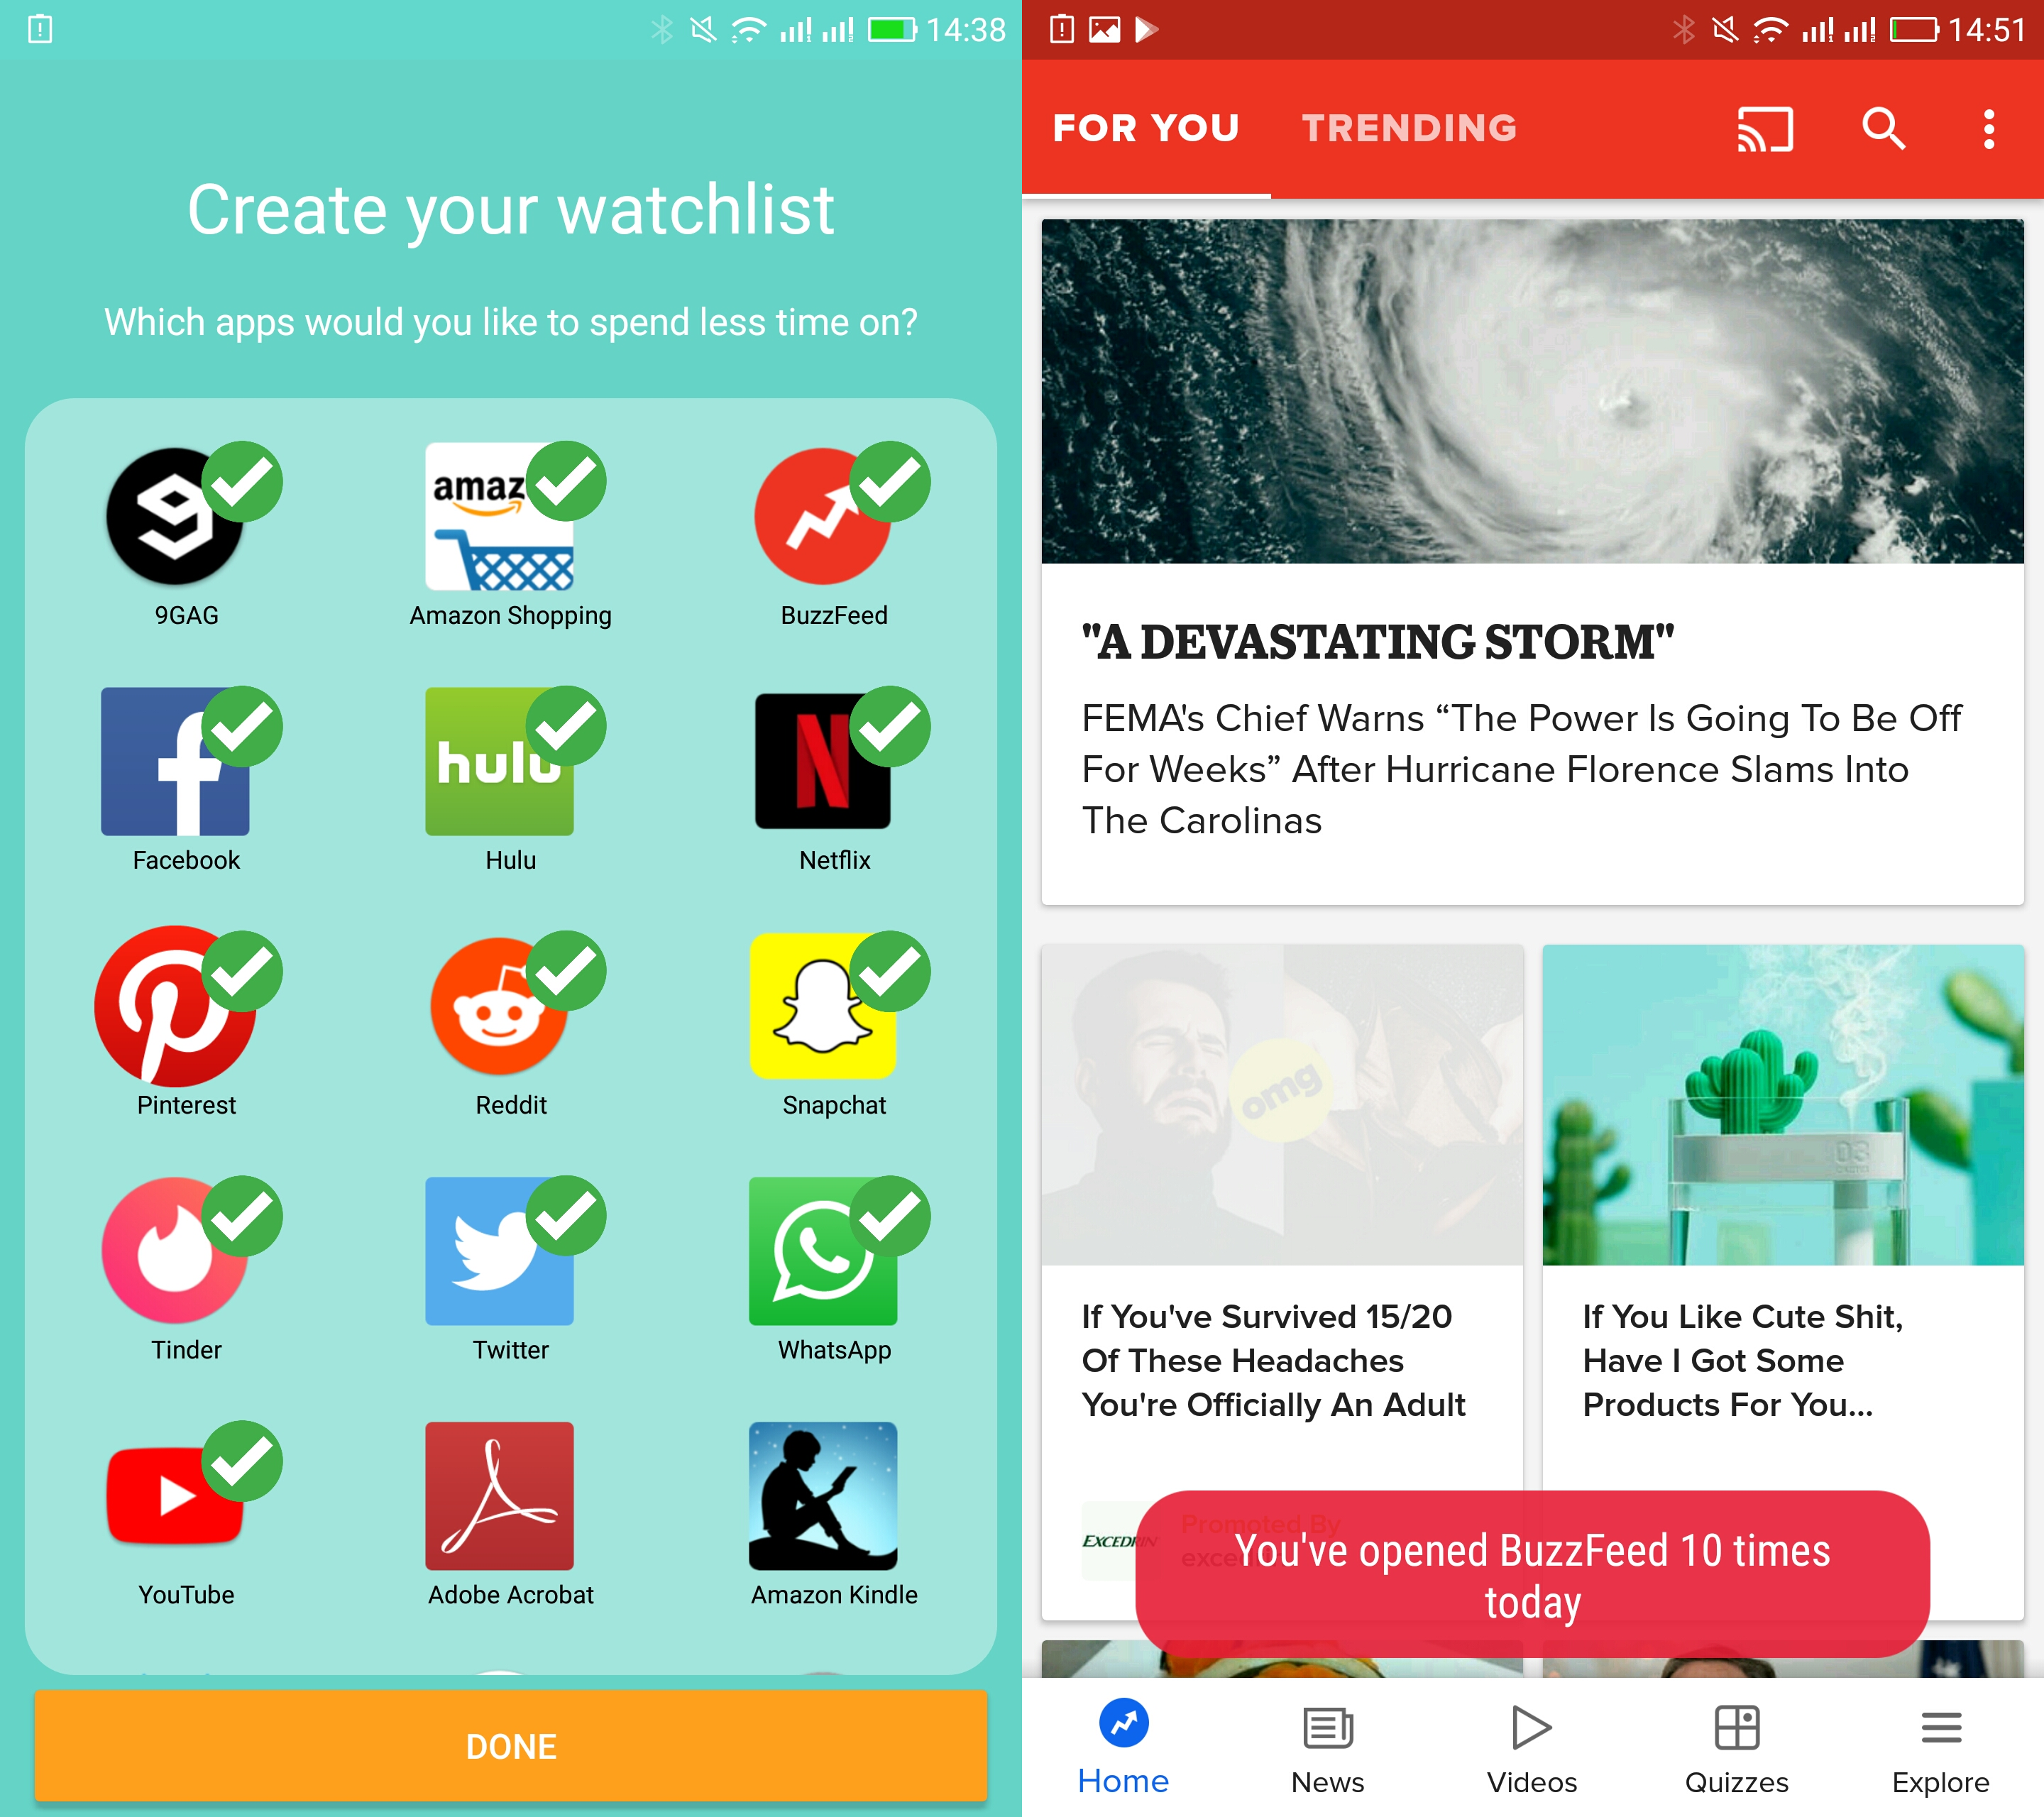
\includegraphics[width=\linewidth]{figures2/android_combined}
\caption{Screenshots from the mobile version of HabitLab.\\
Left: The goal selection screen, where users choose which apps to spend less time on.\\
Right: An example intervention, which shows the visit count when a user opens a goal app. %\msb{save space by cutting the image after the Iqiyi row. No point in having a nearly empty row at the bottom}
}
  \label{fig:android-goal-selection}
\end{figure}

% \begin{figure}
% \begin{minipage}[t]{0.49\linewidth}
% 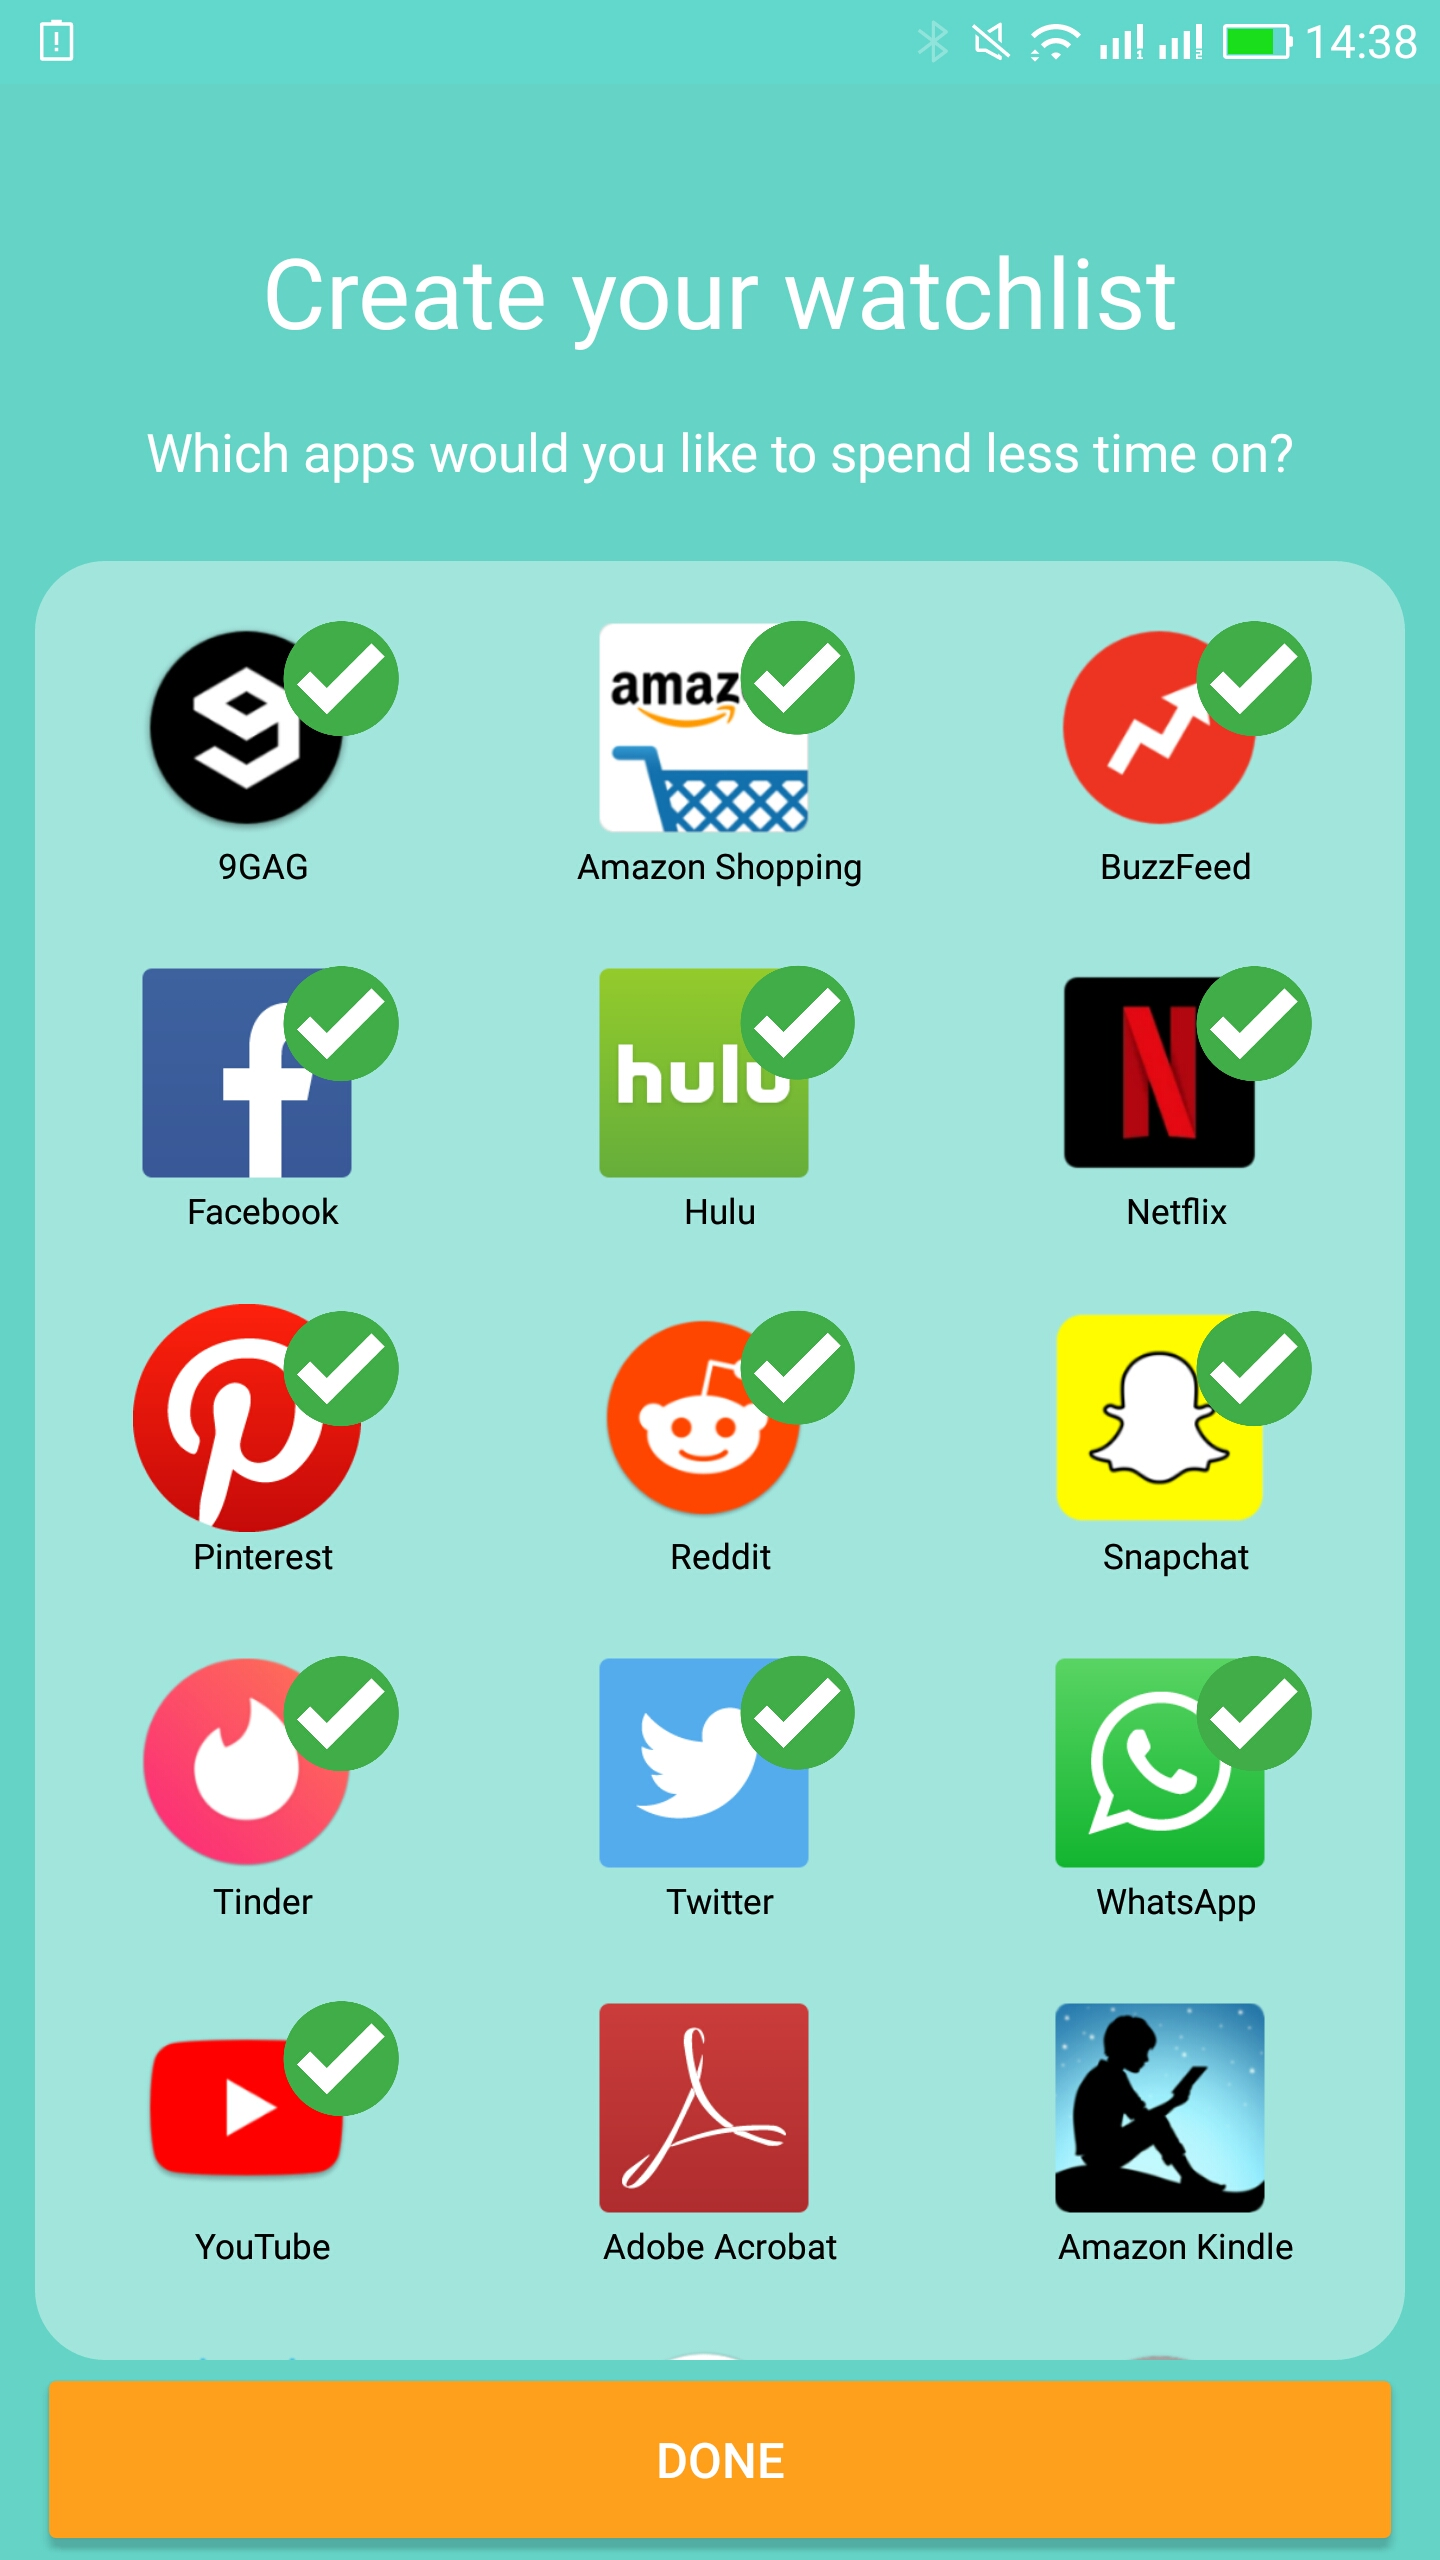
\includegraphics[width=\linewidth]{figures2/android-goal-selection}
% \caption{The goal selection screen, where users choose which apps to spend less time on (mobile version). %\msb{These two mini vertical figures are hard to read. Make it one figure with one caption underneath both.}
% }
%   \label{fig:android-goal-selection}
% \end{minipage}%
% \hfill
% \begin{minipage}[t]{0.49\linewidth}
% 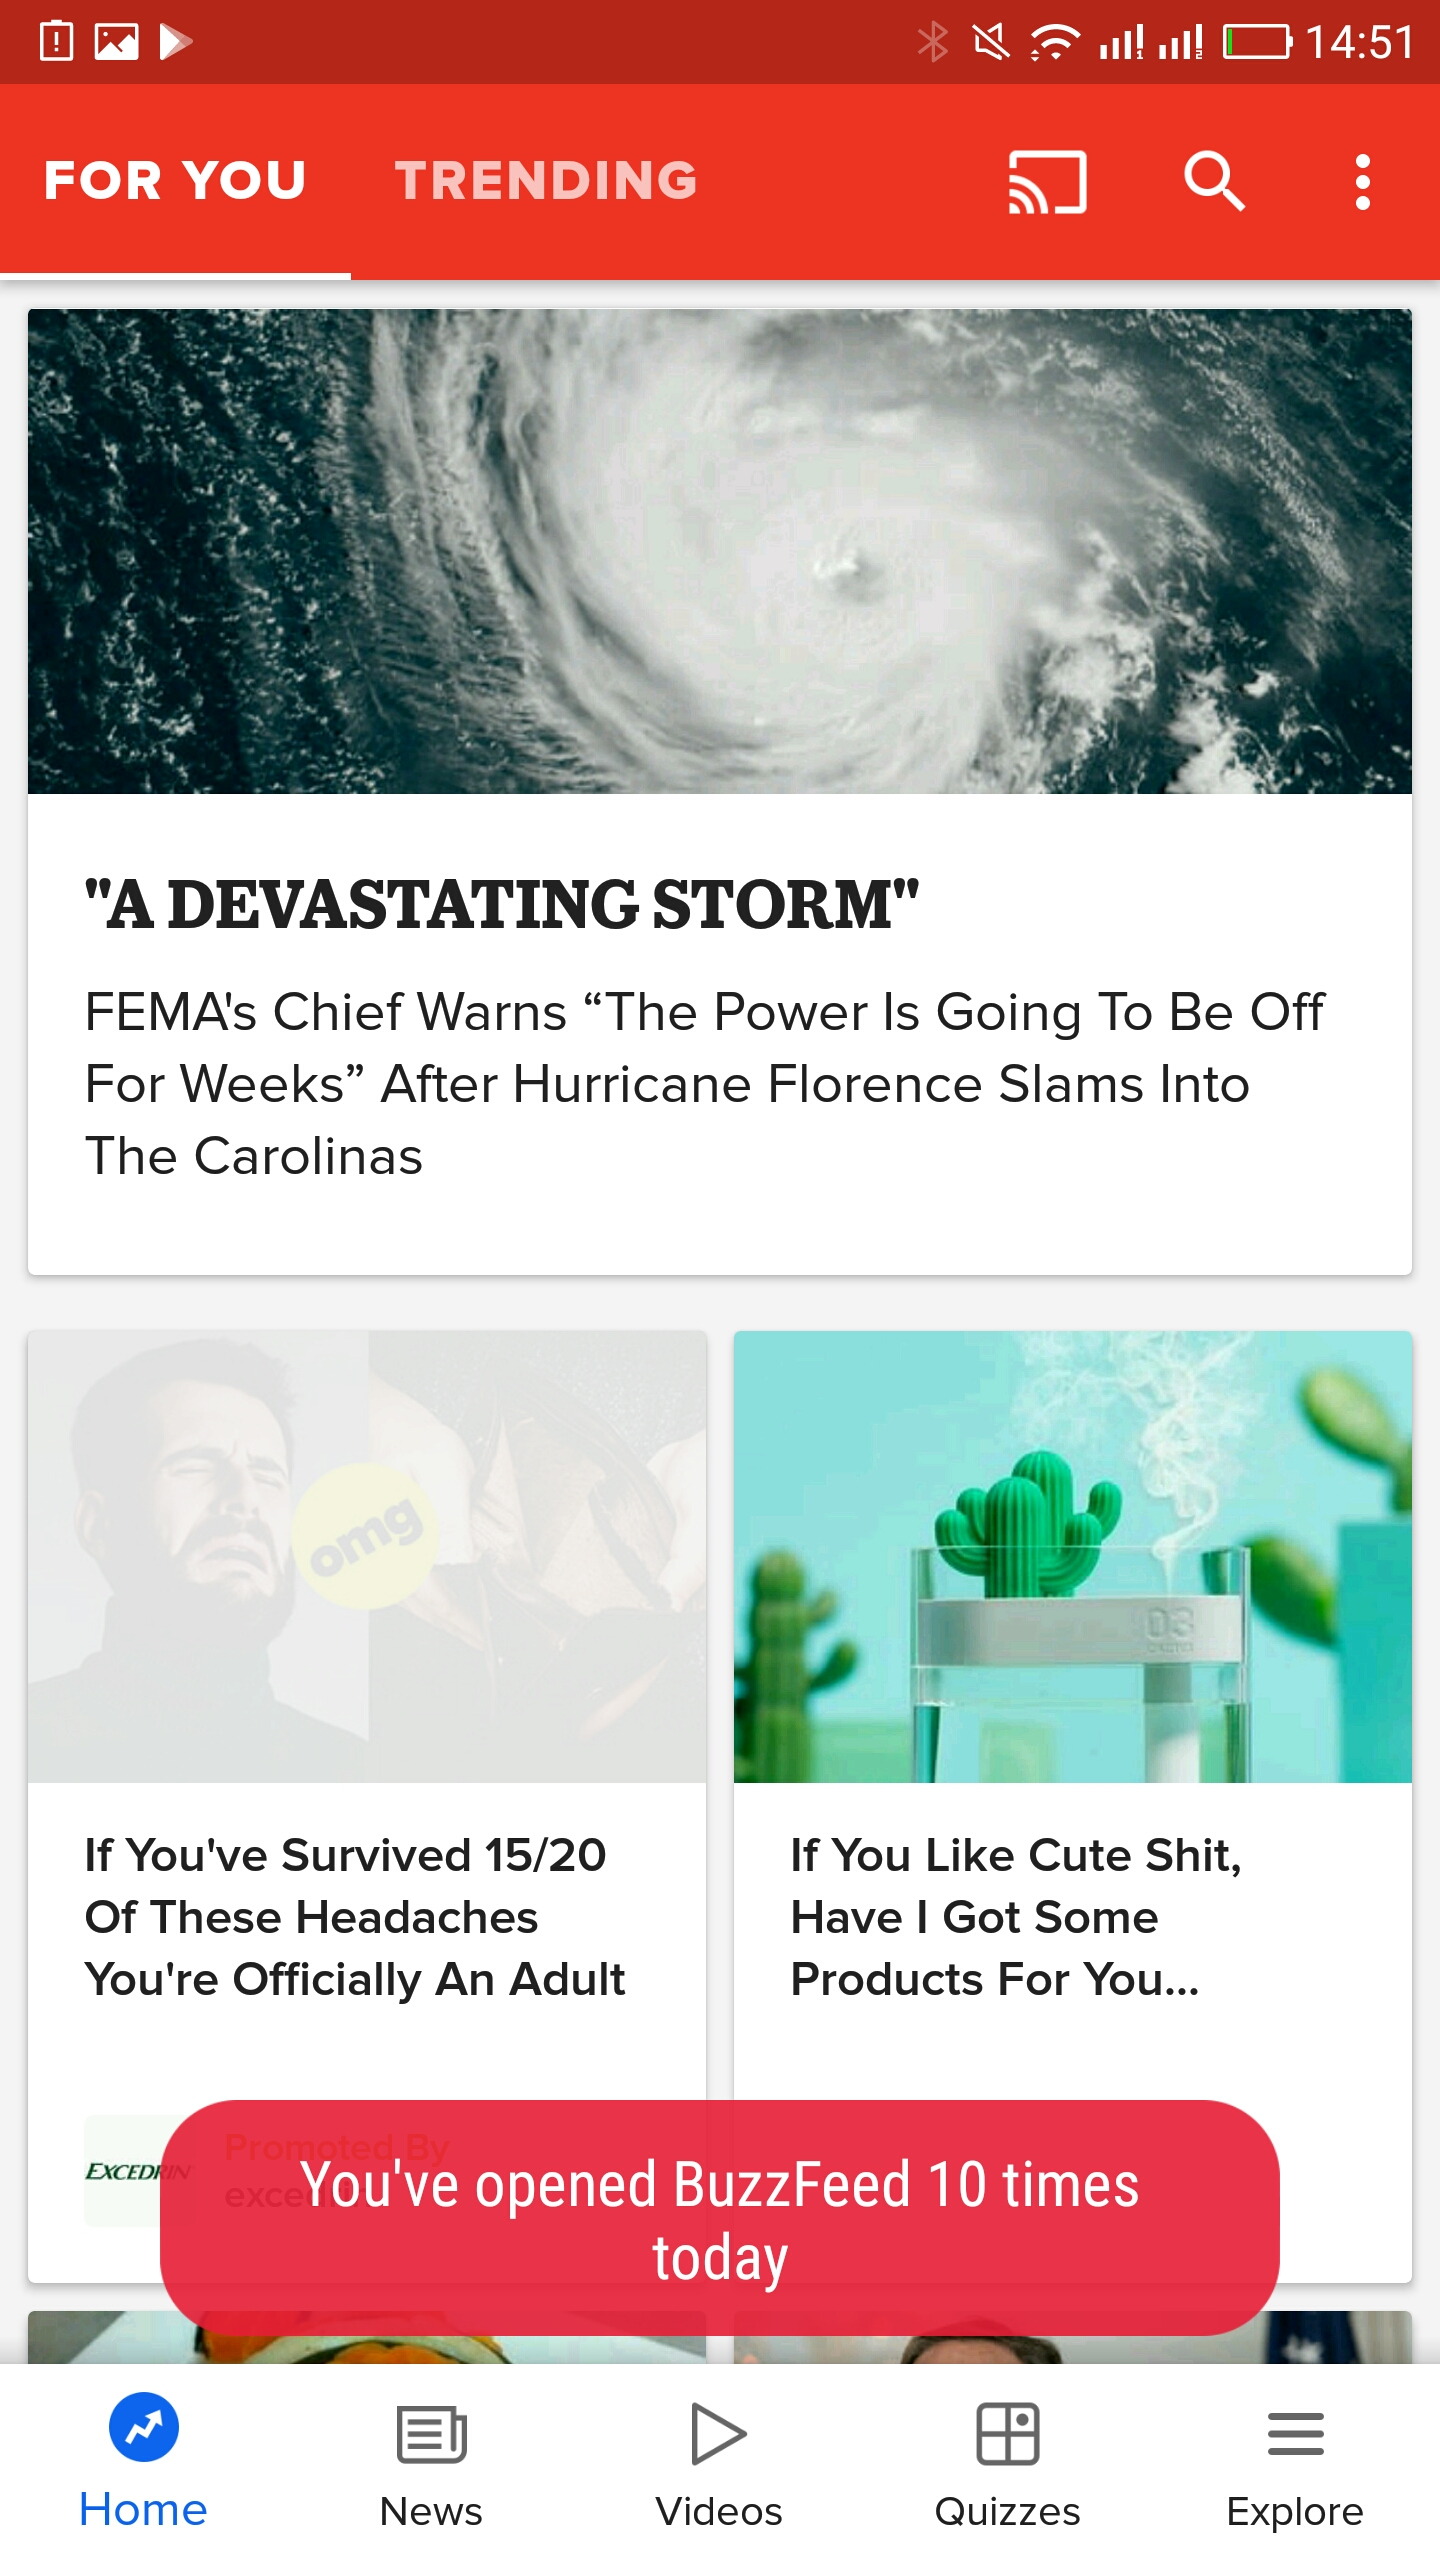
\includegraphics[width=\linewidth]{figures2/android-intervention}
% \caption{An example intervention, which shows the visit count when a user opens an app (mobile version).}
%   \label{fig:android-intervention}
% \end{minipage}
% \end{figure}

% \begin{figure}
% 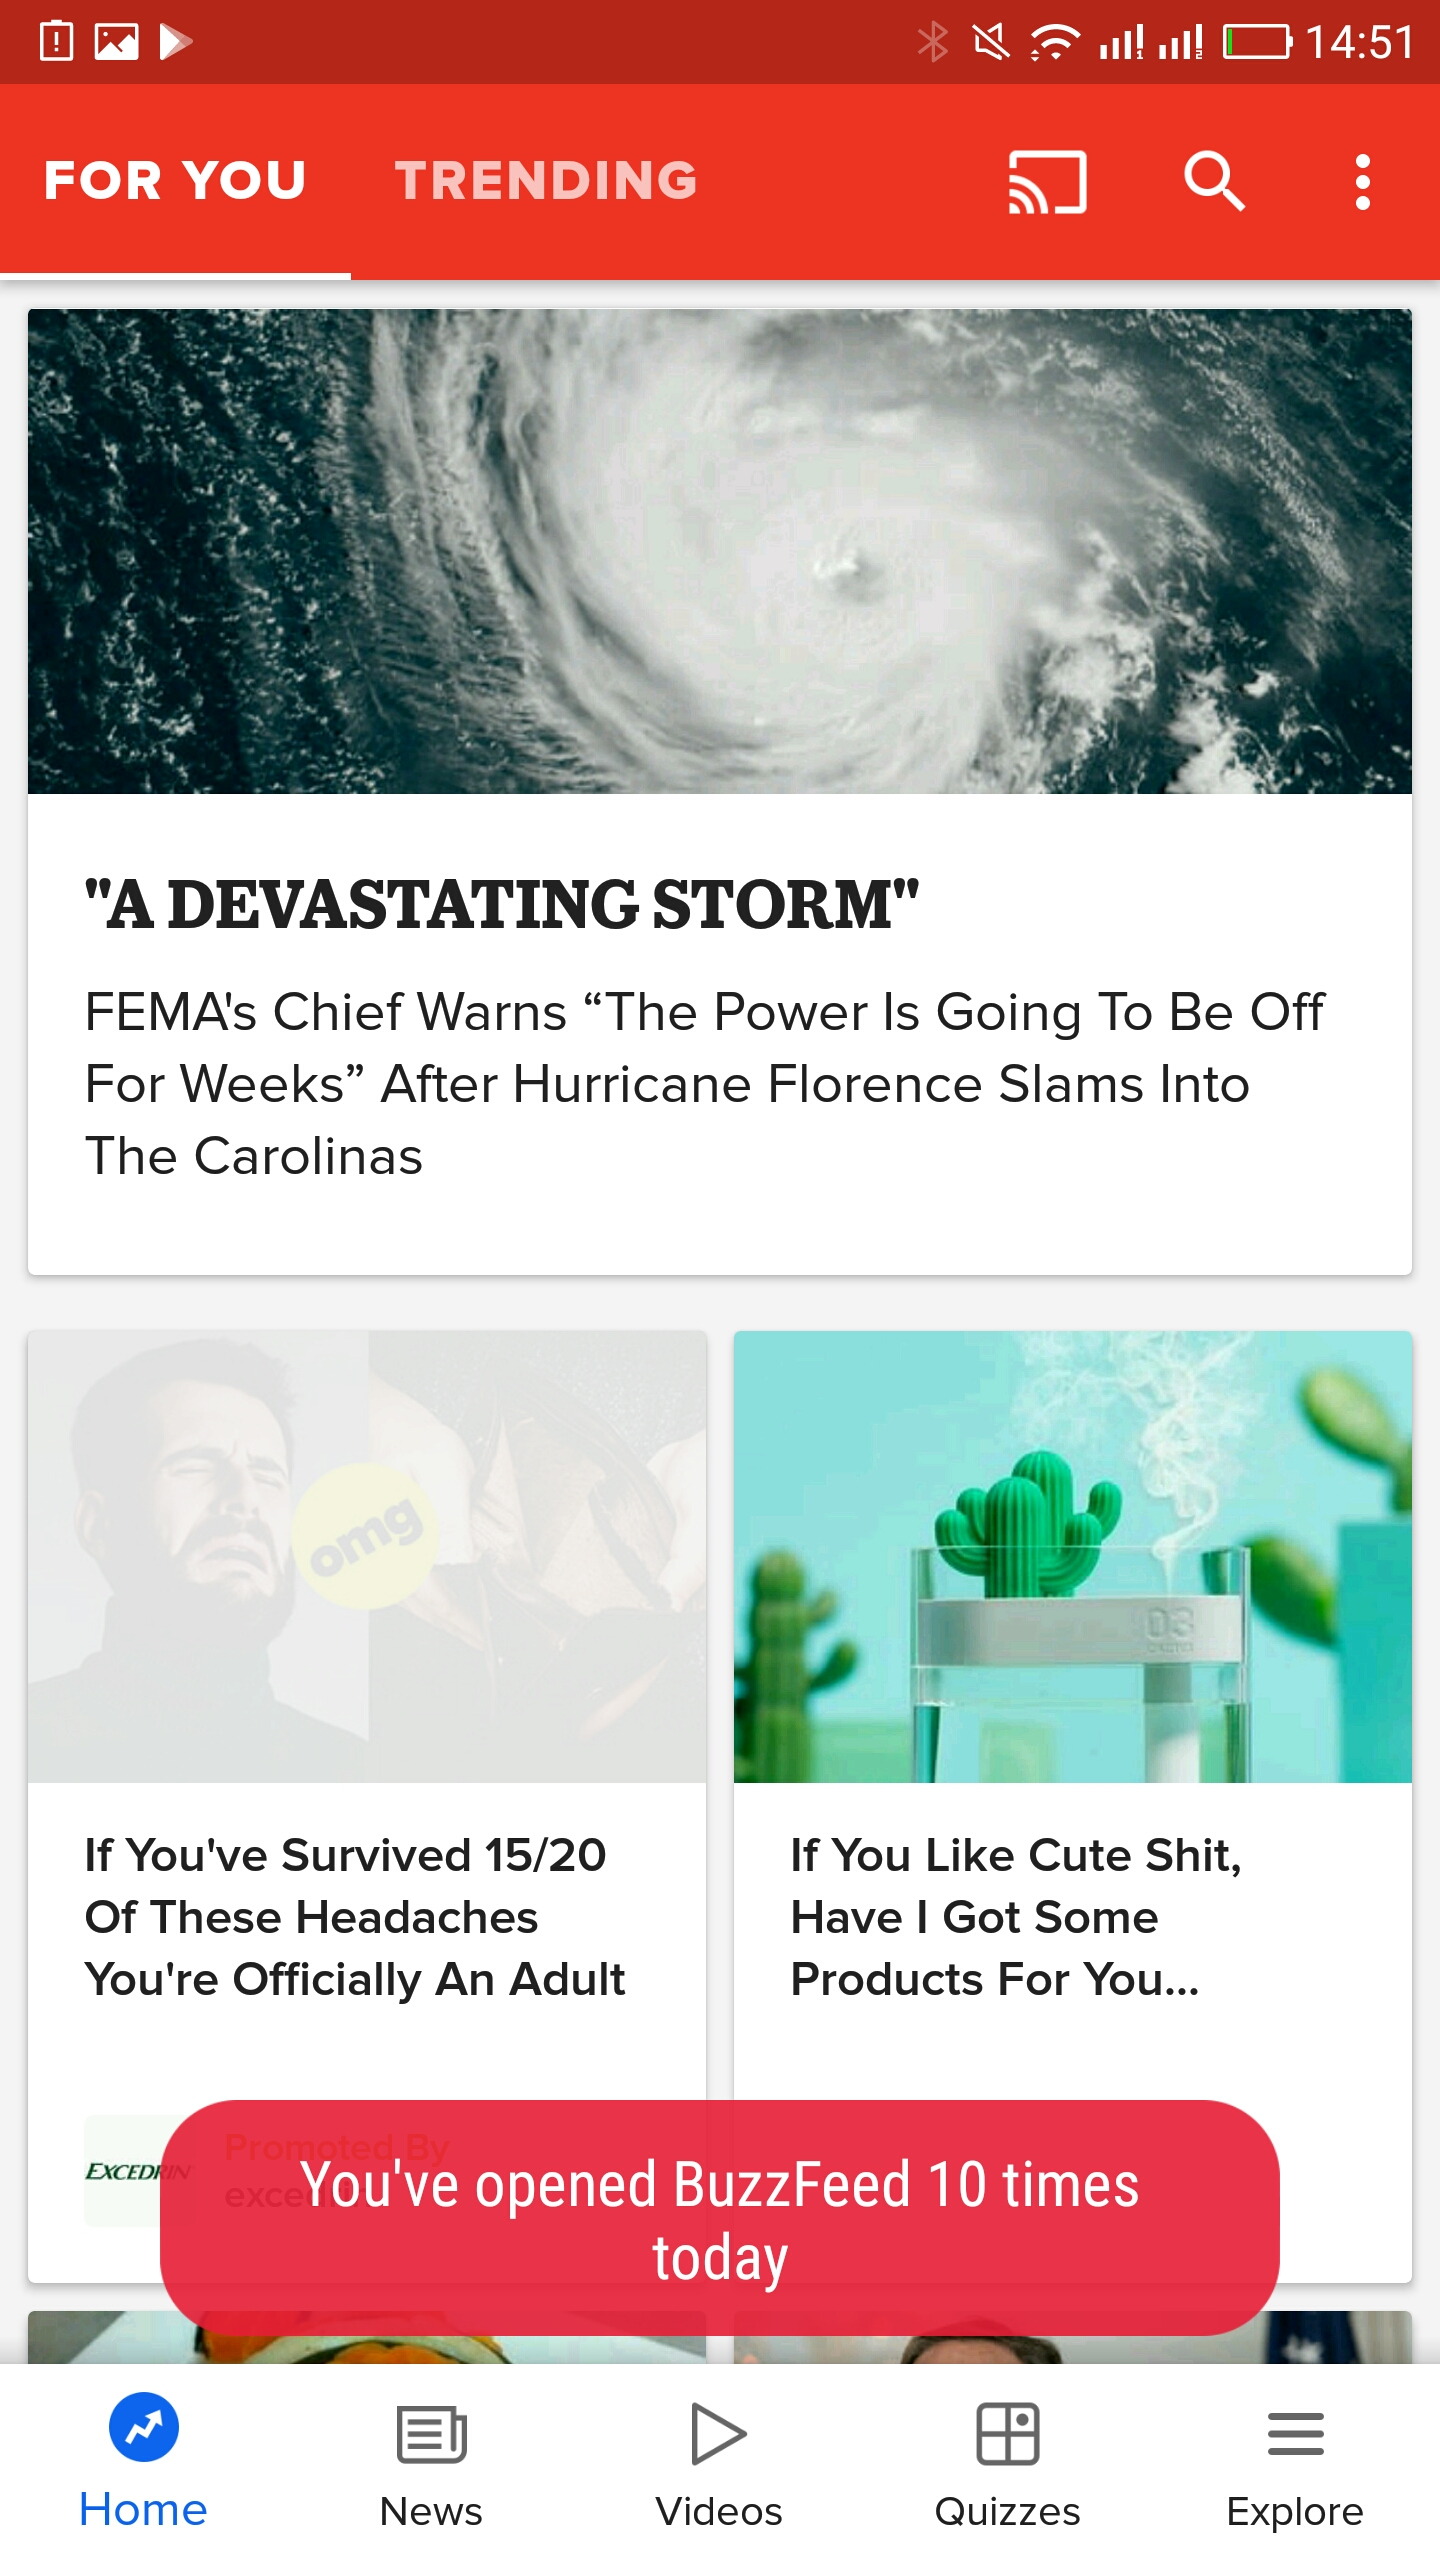
\includegraphics[width=\linewidth]{figures2/android-intervention}
% \caption{Mental model interface: each time the user sees a new intervention, HabitLab names it and explains about rotation.}
%   \label{fig:info}
% \hfill
% \includegraphics[width=\linewidth]{figures2/android-watchlist}
% \caption{User control interface: in addition to the mental model information, HabitLab gives users a direct interface to disable the new intervention.}
%   \label{fig:power}
% \end{figure}

\begin{figure}
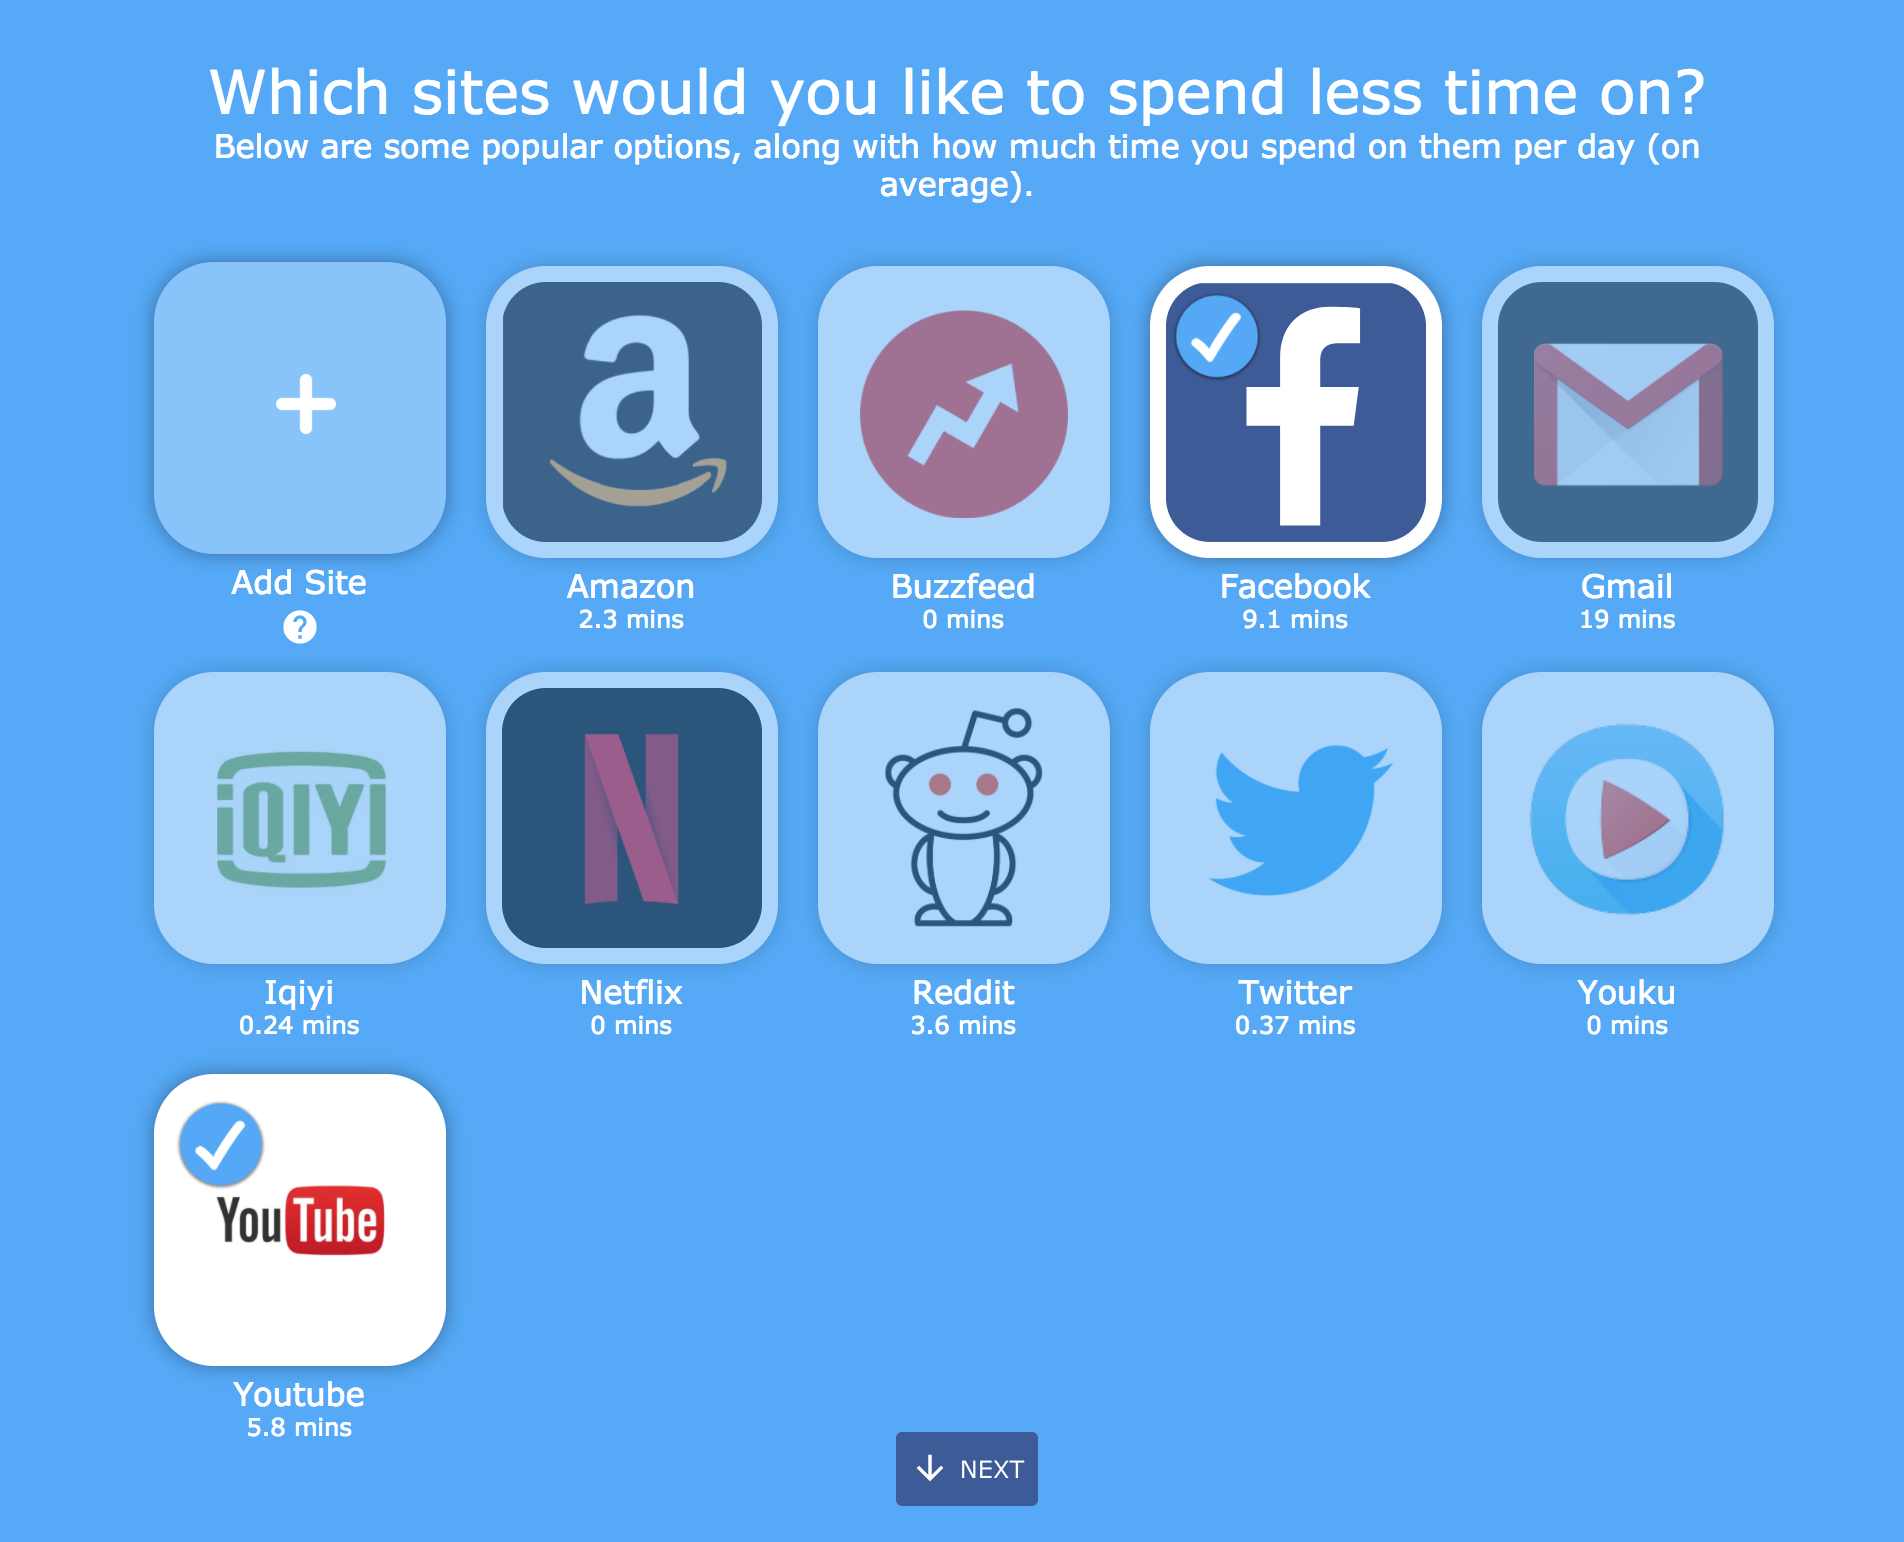
\includegraphics[width=\linewidth]{figures2/chrome-goal-selection}
\caption{The goal selection screen, where users choose which sites to spend less time on (browser version). %\msb{save space by cutting the image after the Iqiyi row. No point in having a nearly empty row at the bottom}
}
  \label{fig:chrome-goal-selection}
\end{figure}

\begin{figure}
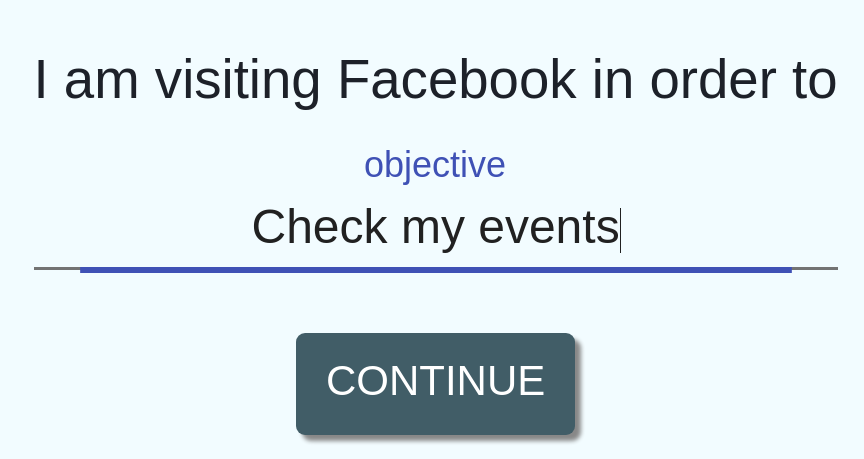
\includegraphics[width=\linewidth]{figures2/chrome-intervention-v3}
\caption{An example intervention, which asks a user to write their objective for visiting a site (browser version). %\msb{This page is really crowded with figures. I suggest moving one onto the next page.} 
% \msb{Save space by reducing this figure to start just above ``I am visiting FB to...''. The turn off button isn't necessary and it adds a ton of space to the paper.}
}
  \label{fig:chrome-intervention}
\end{figure}

Both versions follow the structure of allowing users to choose what they wish to spend less time on (setting goals), and deploying interventions to meet those goals. %The format of the goals differ between the two platforms.
On the Chrome version, users choose sites to spend less time on (goal sites -- for example, \url{facebook.com}), as shown in Figure~\ref{fig:chrome-goal-selection}. On Android, users choose particular apps to spend less time on (goal apps -- for example, the Facebook Android app), as shown in Figure~\ref{fig:android-goal-selection}. Interventions are deployed when users visit a goal site on Chrome (Figure~\ref{fig:chrome-intervention}), and when users open a goal app on Android, as shown in Figure~\ref{fig:android-goal-selection}.

\begin{figure}
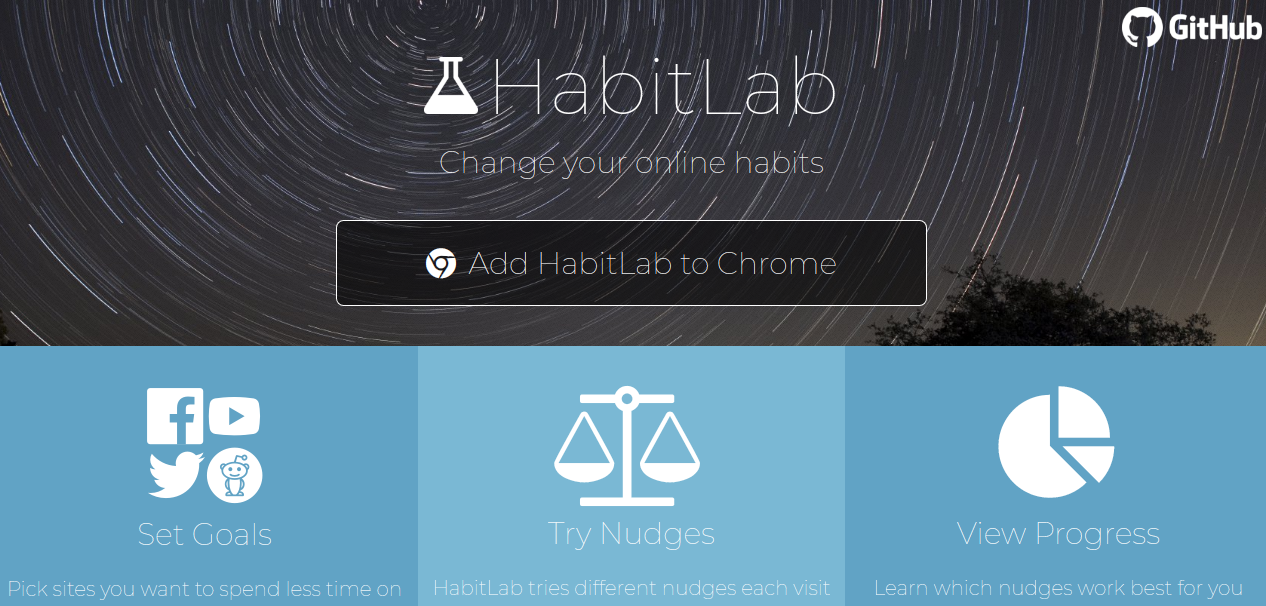
\includegraphics[width=\linewidth]{figures/homepage_cropped}
\caption{HabitLab's homepage describes the browser extension and mobile application. Users adopt it to try out a large number of different possible interventions, called nudges.}
\label{fig:homepage}
\end{figure}

%\section{Browser Version}

\begin{figure}
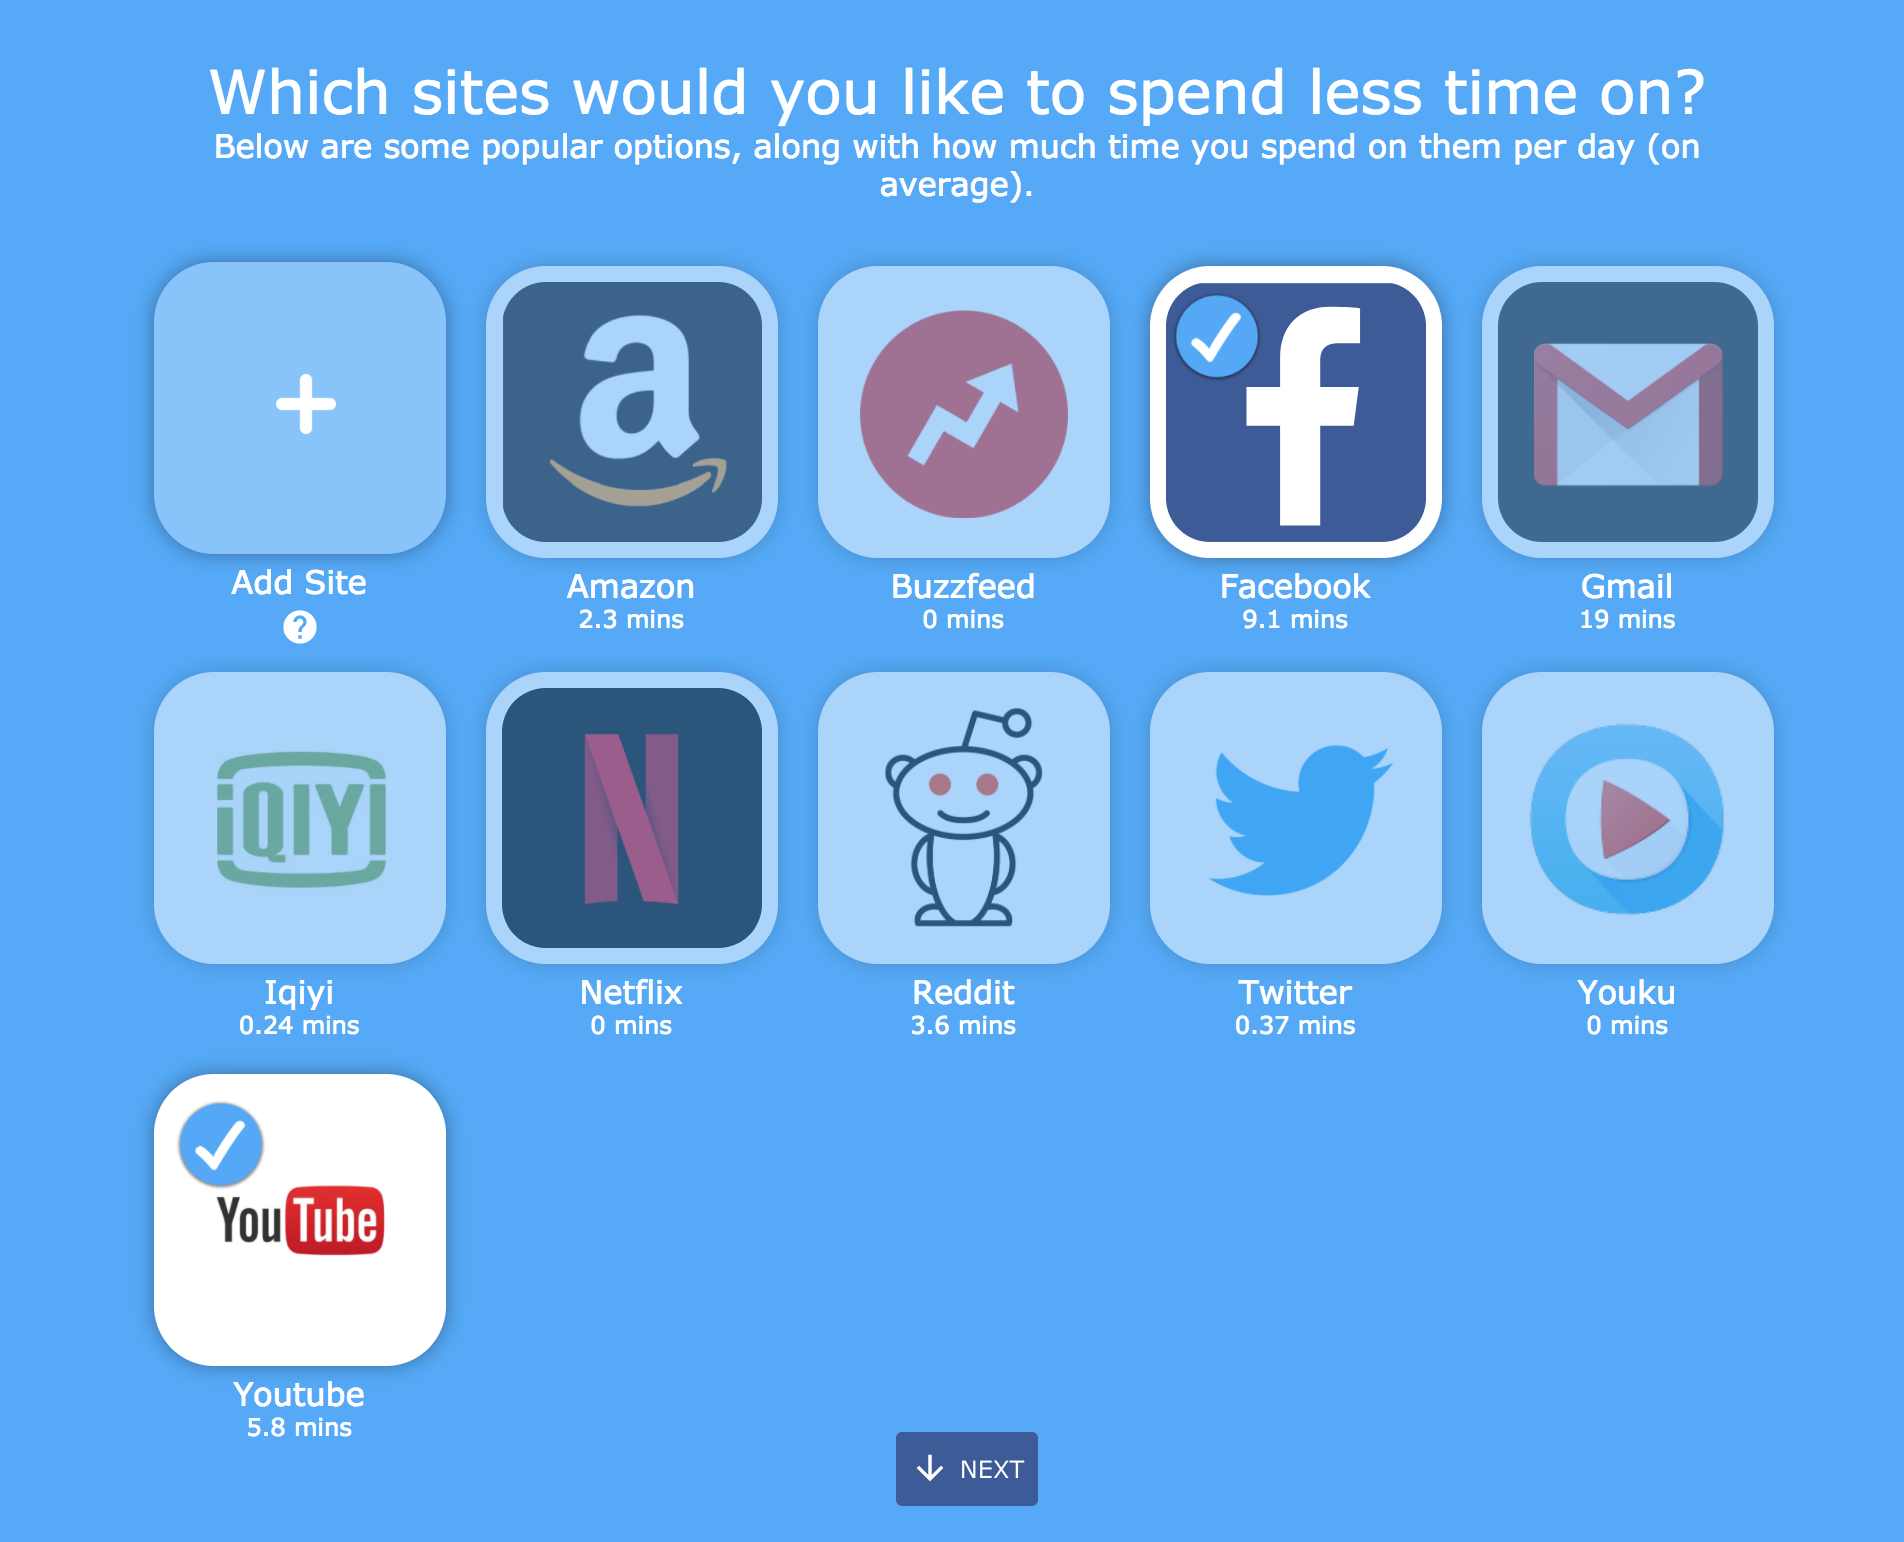
\includegraphics[width=\linewidth]{figures/onboarding_sites}
\caption{During onboarding, users choose which sites they want to spend less time on.}
  \label{fig:onboarding_sites}
\end{figure}

Users install the extension, and go through an onboarding process where they select sites and apps they wish to reduce their time on (Figure~\ref{fig:onboarding_sites}). There are predefined options---Facebook and YouTube are selected by default, as they were the most commonly used---but users can also add any custom site. Custom sites are suggested via an analysis of the user's browsing history. The system explains to users that they will be shown a variety of interventions (Figure~\ref{fig:onboarding_nudges}), a form of self-experimentation~\cite{Karkar:2017:TFS:3025453.3025480}, to help them reduce time on that site. These interventions are typically targeted to each site, for example a news feed blocker for Facebook or a related video hider for YouTube. However, some interventions such as a stopwatch timer can be added to any custom site. Users can preview the interventions for the sites they select, and enable or disable each intervention if desired. Users can later enable or disable interventions and sites through a settings page.

\begin{figure}
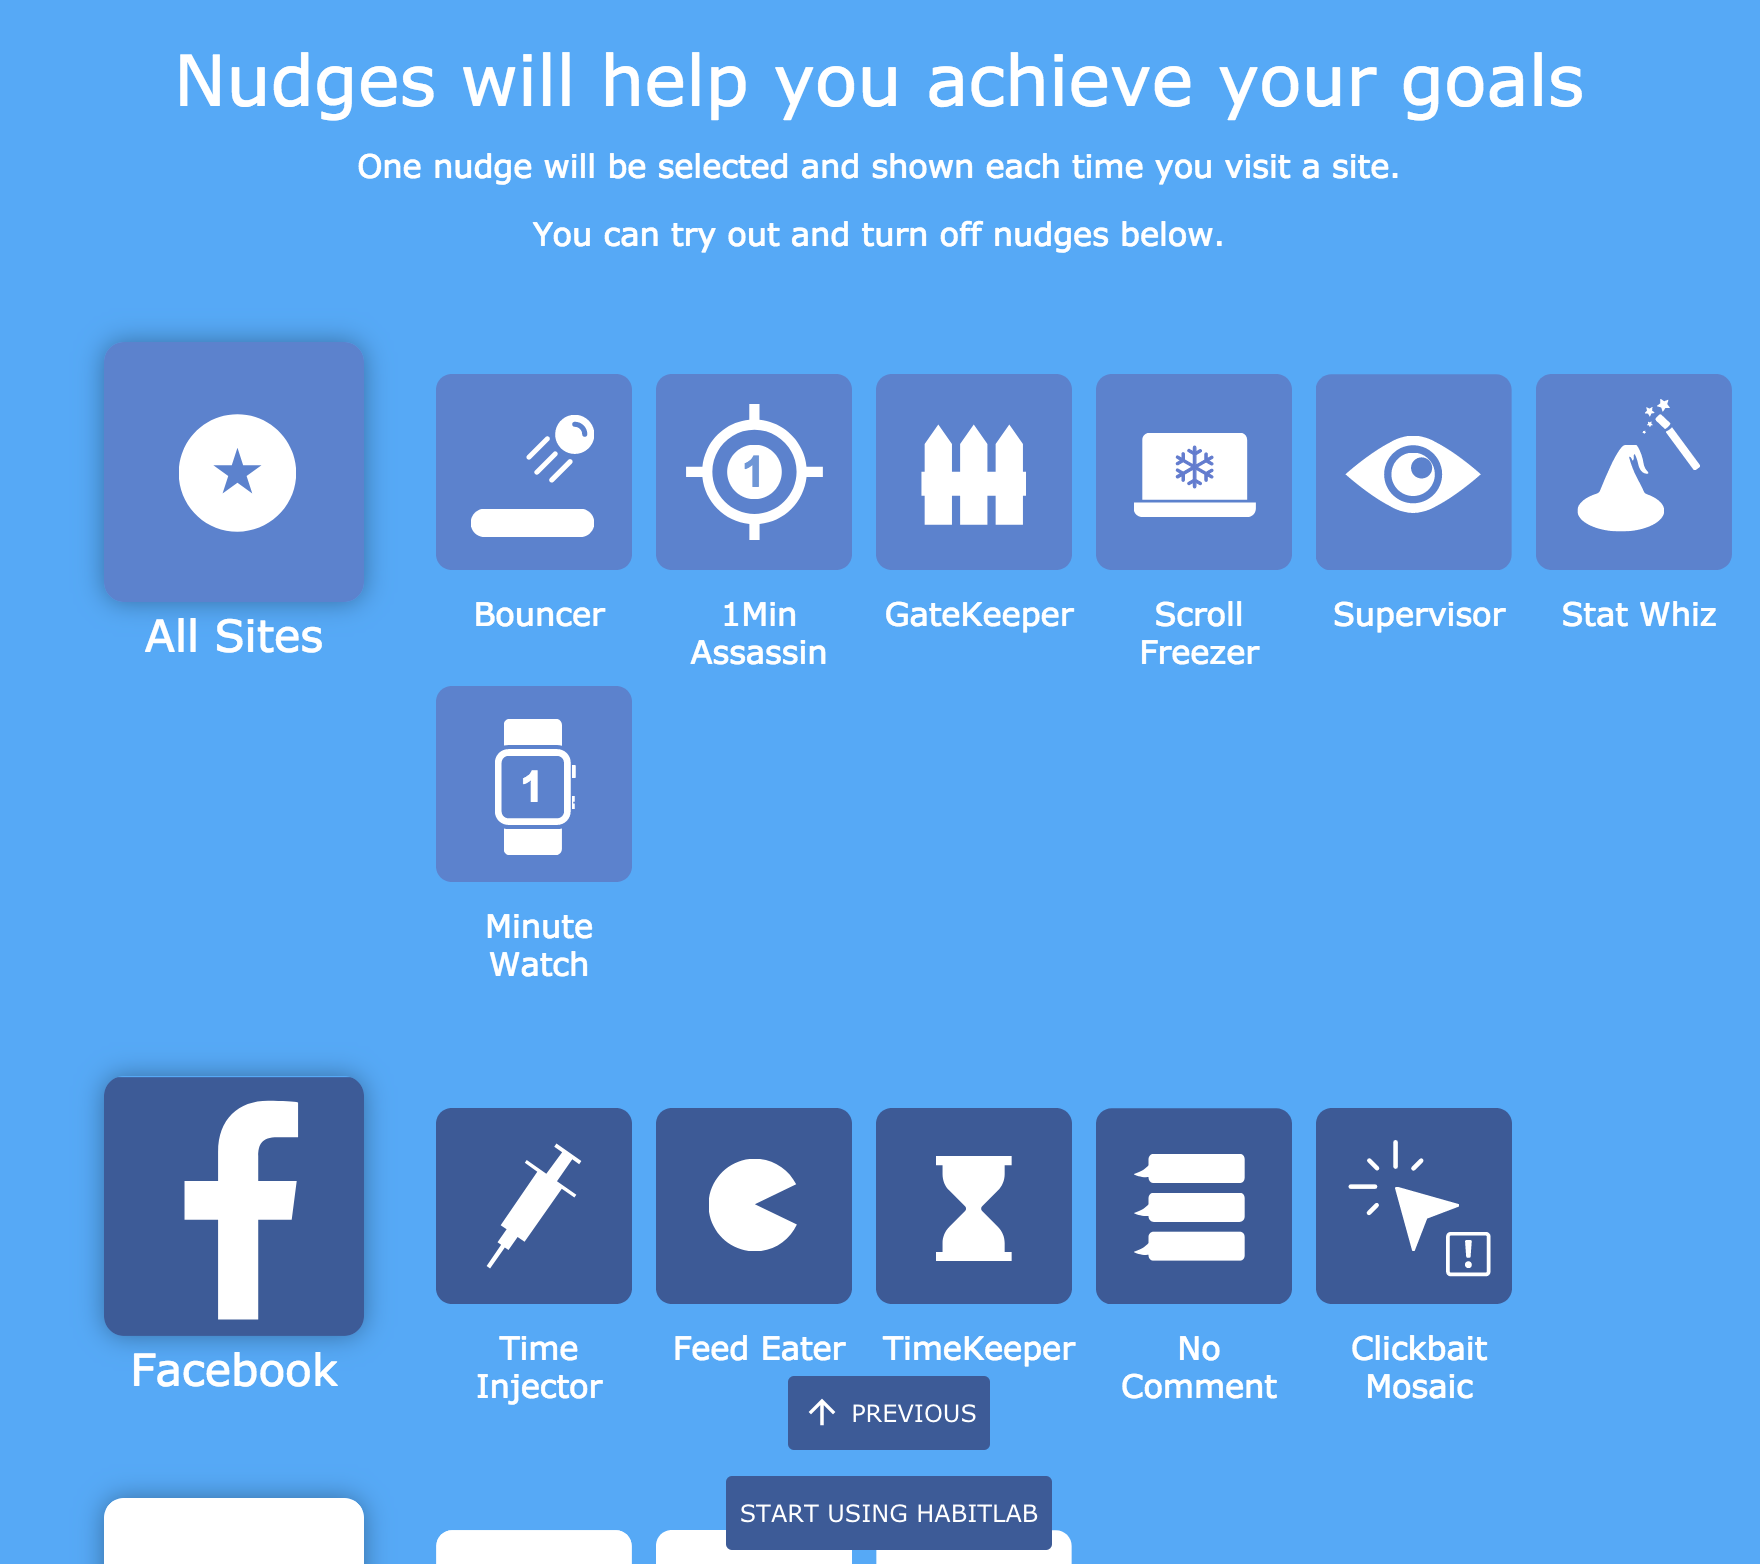
\includegraphics[width=\linewidth]{figures/onboarding_nudges_short}
\caption{Users are presented with the interventions they will see on each site.}
  \label{fig:onboarding_nudges}
\end{figure}

HabitLab emphasizes to users the availability of multiple interventions and that it may show users different interventions each time they load a page. This emphasis is made clear on the HabitLab website, Chrome store listing, and through features in the dashboard such as visualizing the relative effectiveness of different interventions. HabitLab implements a multi-armed bandit algorithm to explore and find the interventions that are most effective for each user, optimizing for minimizing time spent on a site. However, in the experiments in this paper, we disabled this functionality and instead used simple random selection so that we can study the effects of rotation in isolation. \msb{experiments?}

\section{Mobile and Browser Versions}

The Chrome extension and Android app differ in some minor details. They support different sets of goals: users select apps to reduce time on in the Android version, whereas users choose sites to reduce time on in the Chrome version. Additionally, the specific set of interventions available differs between the platforms to fit the design languages of the browser and the mobile phone. The Chrome version has certain interventions which are site-specific -- such as a news feed remover that is specific to Facebook. However, because Android does not allow applications to edit each other's view trees, the Android version's interventions are all glass pane overlays, and thus are general and can be used on any app. The concept of a session is different on the platforms: in the Chrome version, a session is time on a site until that tab is either closed or the user goes to a different domain. Time measured is active time -- so if the tab is not focused, or if there is no keyboard or mouse activity for over a minute, the timer is temporarily paused. However, on Android, because there is no concept of a tab, the measurement of a session is different. There, a session is considered the duration over which an app is opened and focused. Closing the app, switching to a different app, or turning off the phone will end the current session.

\section{Design of HabitLab Interventions}

HabitLab can track time and deploy interventions on all sites, but some interventions are tailored towards specific sites. There are 27 interventions total: seven generic interventions that can be used on all sites, five interventions designed specifically for Facebook, and additional ones designed specifically for YouTube, Reddit, Twitter, Netflix, Gmail, Amazon, iQiyi, and Youku.

Interventions are designed drawing on theories of behavior change---for example, goal setting theory~\cite{locke2002building}, persuasion~\cite{cialdini1987influence,fogg2002persuasive,abraham2008taxonomy}, and gamification~\cite{deterding2011game}. A sample of the interventions available for Facebook, categorized according to underlying strategies and theories, are shown in Table~\ref{tab:theories}. Screenshots of some Facebook interventions are shown in Figure~\ref{fig:interventions}.  Descriptions of the interventions on the Chrome and Android versions can be found at the end of this chapter. %\msb{always use non breaking space \~ between Figure and number, and between sentence and citation block}
% , and health ~\cite{abraham2008taxonomy} \msb{health is not a theory of behavior change}

%The design of HabitLab's interventions is based on theories such as Cialdini's factors of influence~\cite{cialdini1987influence} and the behavior change wheel taxonomy of behavior change interventions~\cite{abraham2008taxonomy}. Description of the interventions on the Chrome and Android versions can be found in the Appendix.

Not all interventions are enabled by default---this is because some of them have higher attrition rates than others. Non-default interventions can be previewed and enabled by users during onboarding and on the settings page. The interventions enabled by default were the ones we found to have low attrition rates during pilot deployments---we chose this strategy to ensure user retention and growth, which is a prerequisite for gathering data in an in-the-wild experiment setting.

\begin{table}[tb]
\small
\begin{center}
\begin{tabular}{ p{3.3cm} p{3.4cm} p{6.2cm} }
  \textbf{Strategy} & \textbf{Theory} & \textbf{Intervention} \\
  %\hline
  Commitment & Self-consistency theory~\cite{allgeier1979waffle,cialdini1987influence,sherman1980self} & Ask the user to set a goal for the length of time they will stay on the site (generic) \\
  Enforce default limits & Status quo bias ~\cite{samuelson1988status} & Automatically close tab after 60 seconds unless the user clicks a button to ask for more time (generic) \\
%  Enforce default limits & Status quo bias ~\cite{samuelson1988status} & Prevents scrolling unless the user clicks a button to continue scrolling (generic) \\
Reduce social incentives & Social proof~\cite{sherif1935study,cialdini1987influence} & Hide Facebook comments by default (default) \\
  Delaying Rewards & Operant conditioning~\cite{baron1991analyzing} & Make the user wait 10 seconds before visiting Facebook (generic) \\
%  Delaying Rewards & Operant conditioning~\cite{baron1991analyzing} & Shows a page with time spent on Facebook today which they need to click through to get to Facebook (generic) \\
Removing Rewards & Operant conditioning~\cite{baron1991analyzing} & Hide the news feed (default) \\
%  Removing Rewards & Operant conditioning~\cite{baron1991analyzing} & Hide videos and clickbait in the news feed \\
% Gamification & Goal setting theory~\cite{locke2002building}, Flow~\cite{csikszentmihalyi1996flow} & Get points and badges for seeing fewer newsfeed items  \\
  Inform the user & Theory of reasoned action~\cite{ajzen1977attitude} & Show a counter at the top of the page of how long user has been on Facebook today (default, generic) \\
%  Inform the user & Theory of reasoned action~\cite{ajzen1977attitude} & Show a toast notification each minute displaying how long they've been on Facebook today (default, generic) \\
%  Inform the user & Theory of reasoned action~\cite{ajzen1977attitude} & Show a desktop notification each minute displaying how long they've been on Facebook today (generic) \\
% Inform the user & Theory of reasoned action~\cite{ajzen1977attitude} & Inject messages into the news feed showing how long they've been on Facebook today (default) \\
  %Make a plan & Theory of planned behavior \cite{gollwitzer1999implementation} & Ask the user to write out a concrete plan for how they will avoid coming back to the site next time they are tempted to do so \\
  % Rewards/punishment & Operant conditioning~\cite{baron1991analyzing} & Block the site for four hours if the user spends too much time on site in this session \\
  %Stress management & Stress coping~\cite{thoits1995stress} & Reflection on stressors that lead to visiting Facebook \\
  
\end{tabular}
\end{center}
%\vspace{-.7em}
\caption{A subset of the interventions for Facebook, categorized according to persuasion strategy and theory. Interventions that are enabled by default are marked \textit{default}, interventions that are available for all sites are marked \textit{generic}.}
\label{tab:theories}
\end{table}


% todo need to retake these screenshots so they're anonymous
\begin{figure}
	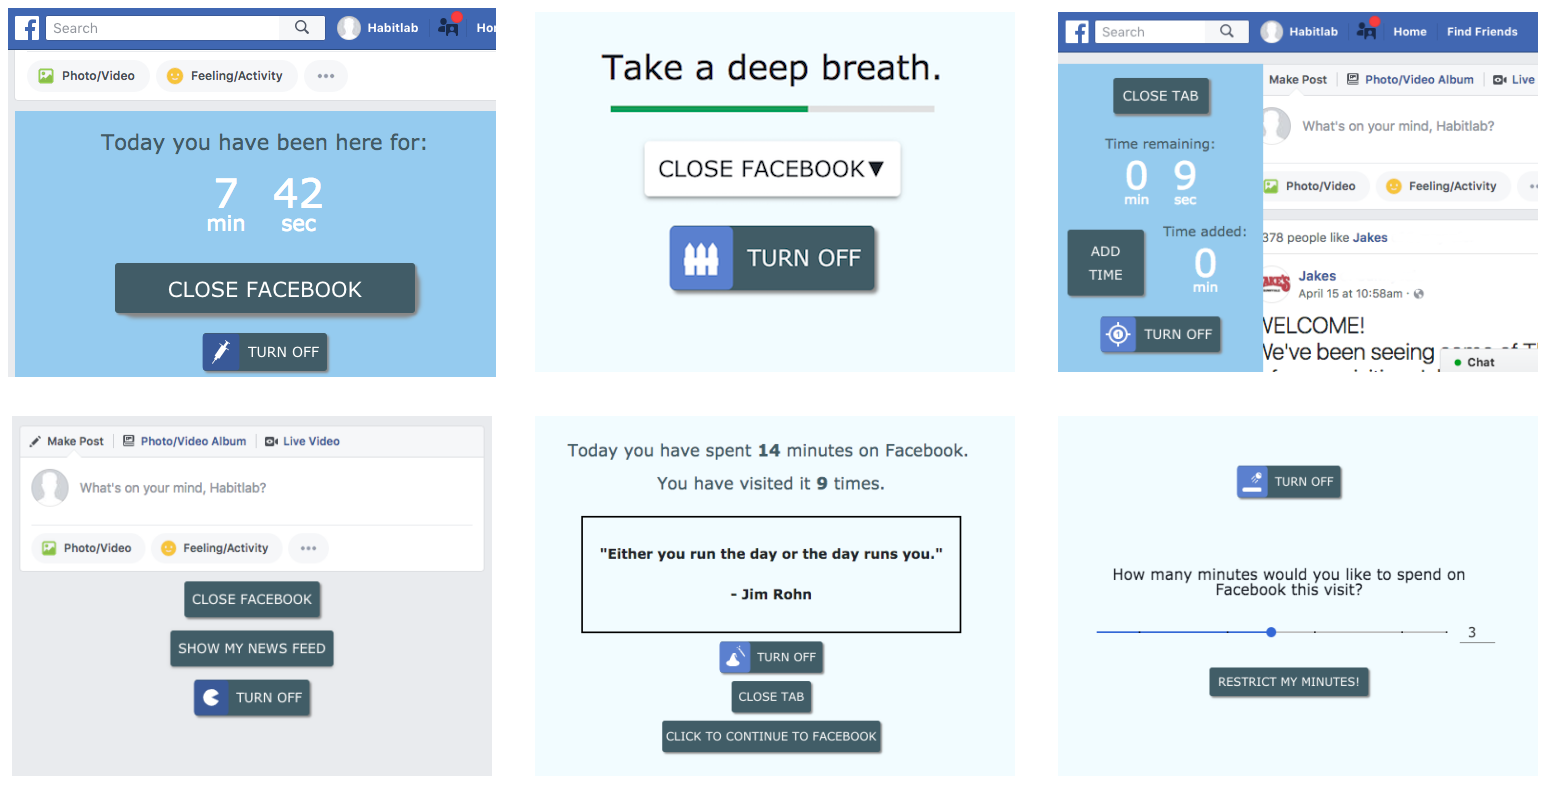
\includegraphics[width=1.0\textwidth]{figures/interventions_new.png}
	\caption{Examples of interventions available for reducing time on Facebook. From left to right, top to bottom: a timer injected into the news feed; a page before opening Facebook requiring that the user wait a few seconds before visiting; a countdown timer that automatically closes the tab after time elapses; an opt-in required to show the news feed; an interstitial page before opening Facebook with a quote; an interstitial page before opening Facebook that requires the user set a time limit for how long they will spend this session.}
\label{fig:interventions}
\end{figure}

\section{HabitLab adoption and user demographics}

As of writing, the browser version of HabitLab has over 12,000 daily active users, and the Android version has over 500 daily active users.

% todo need to retake these screenshots so they're anonymous
\begin{figure}
	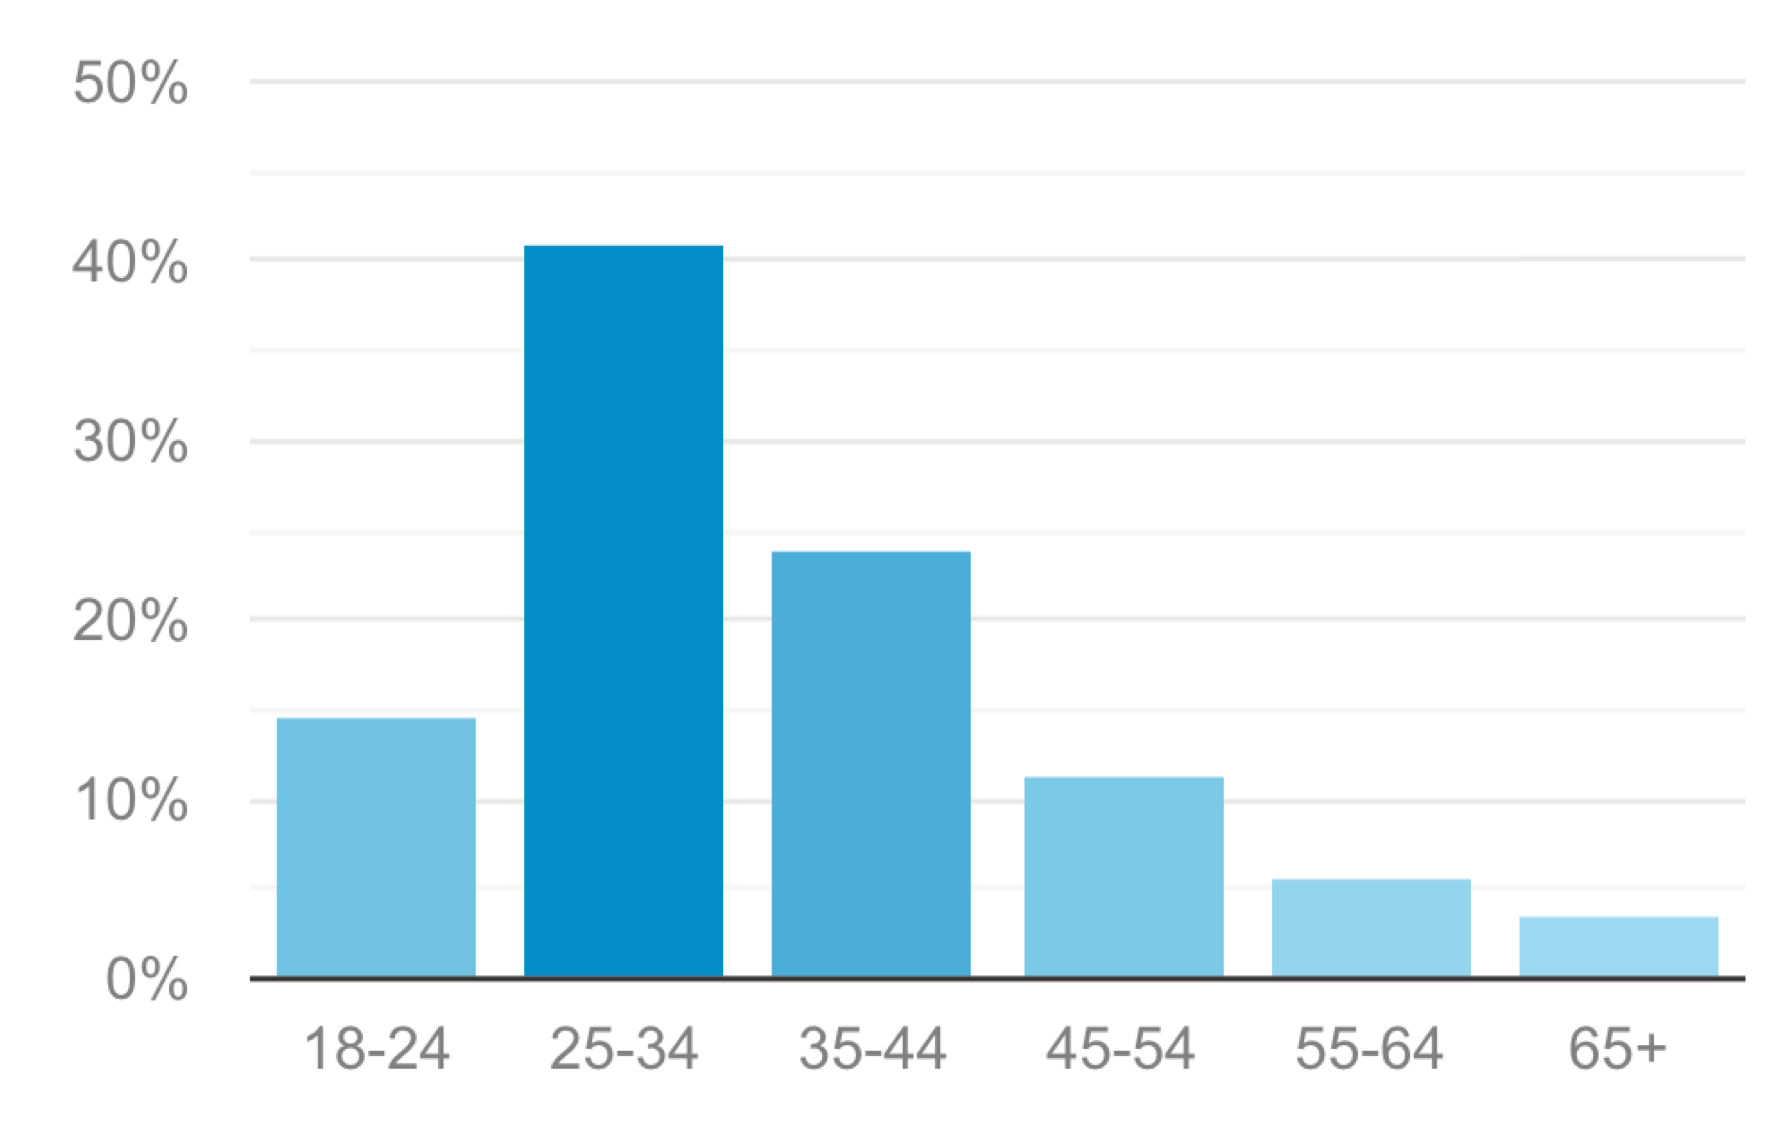
\includegraphics[width=1.0\textwidth]{figuresS/user_ages.png}
	\caption{Ages of HabitLab users. 25-35 is the most-represented demographic.}
\label{fig:user_ages}
\end{figure}

Demographics according to Google Analytics indicate that our users are 81\% male, with the most commonly represented age group being 25-34, as shown in \ref{fig:user_ages}.

% todo need to retake these screenshots so they're anonymous
\begin{figure}
	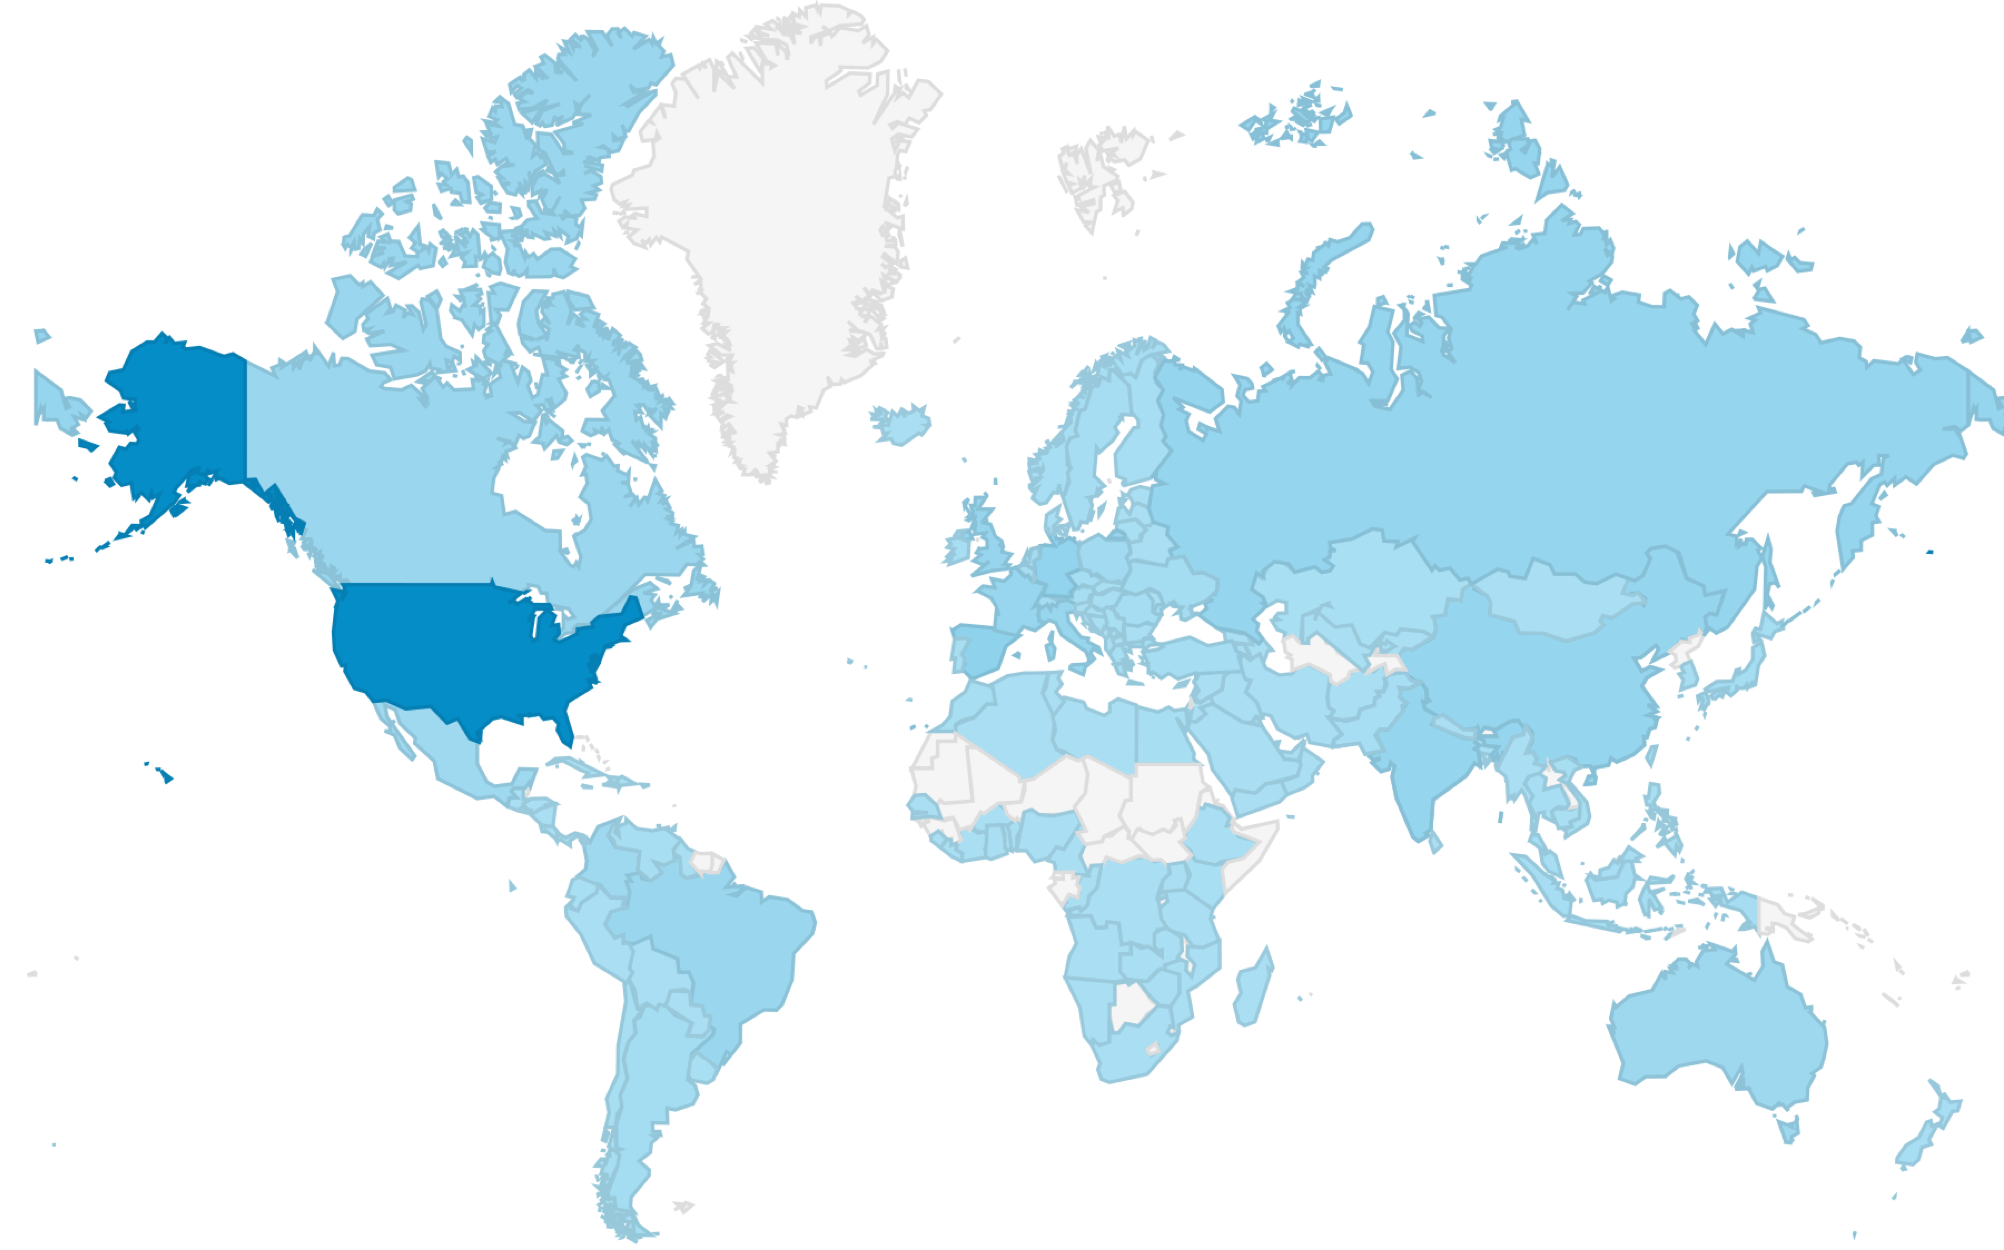
\includegraphics[width=1.0\textwidth]{figuresS/user_map.png}
	\caption{Map of countries representing HabitLab users. North America, Europe, and Asia are all well-represented.}
\label{fig:user_map}
\end{figure}

Our userbase represents a diverse set of countries and languages -- users represent 151 countries as shown in \ref{fig:user_map}. The top 10 countries are shown in \ref{fig:user_countries} -- the US is the most-represented country, representing 30\% of the userbase.

% todo need to retake these screenshots so they're anonymous
\begin{figure}
	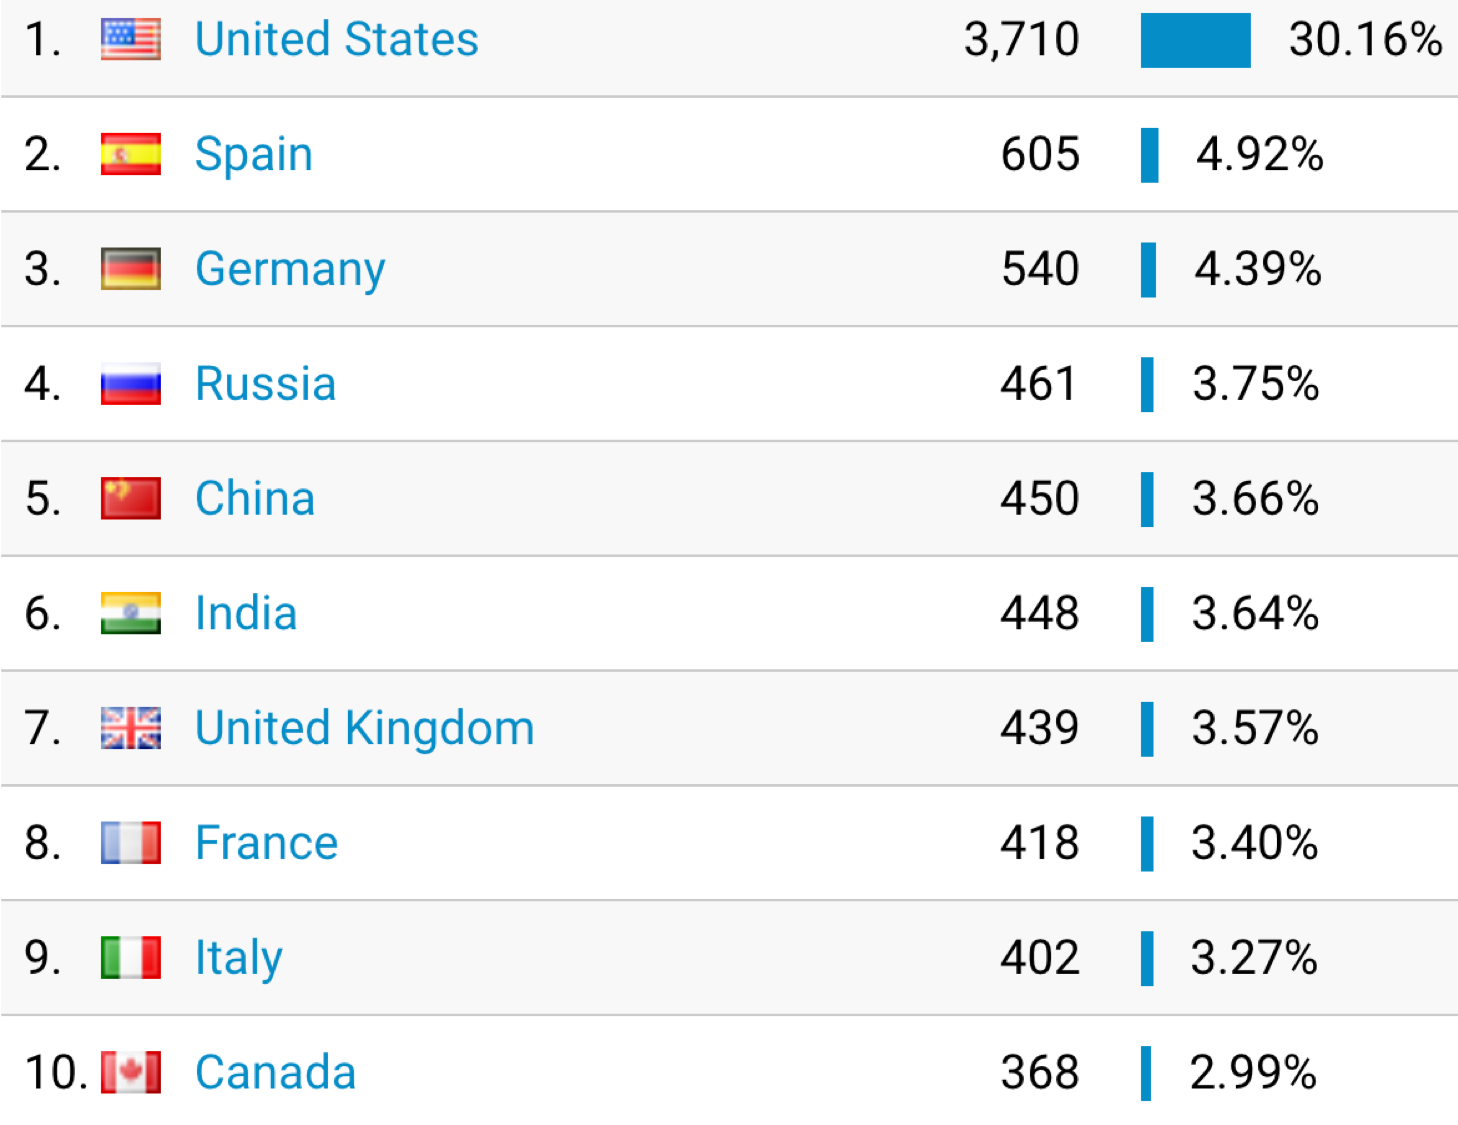
\includegraphics[width=1.0\textwidth]{figuresS/user_countries.png}
	\caption{Top 10 countries using HabitLab. Users from the US account for 30\% of our userbase.}
\label{fig:user_countries}
\end{figure}

Half of our userbase uses English as their preferred language for displaying webpages, as indicated in \ref{fig:user_languages}. Volunteers have translated HabitLab into 13 languages (Arabic, Chinese, Czech, Dutch, French, German, Greek, Italian, Polish, Portuguese, Russian, Spanish, and Turkish).

% todo need to retake these screenshots so they're anonymous
\begin{figure}
	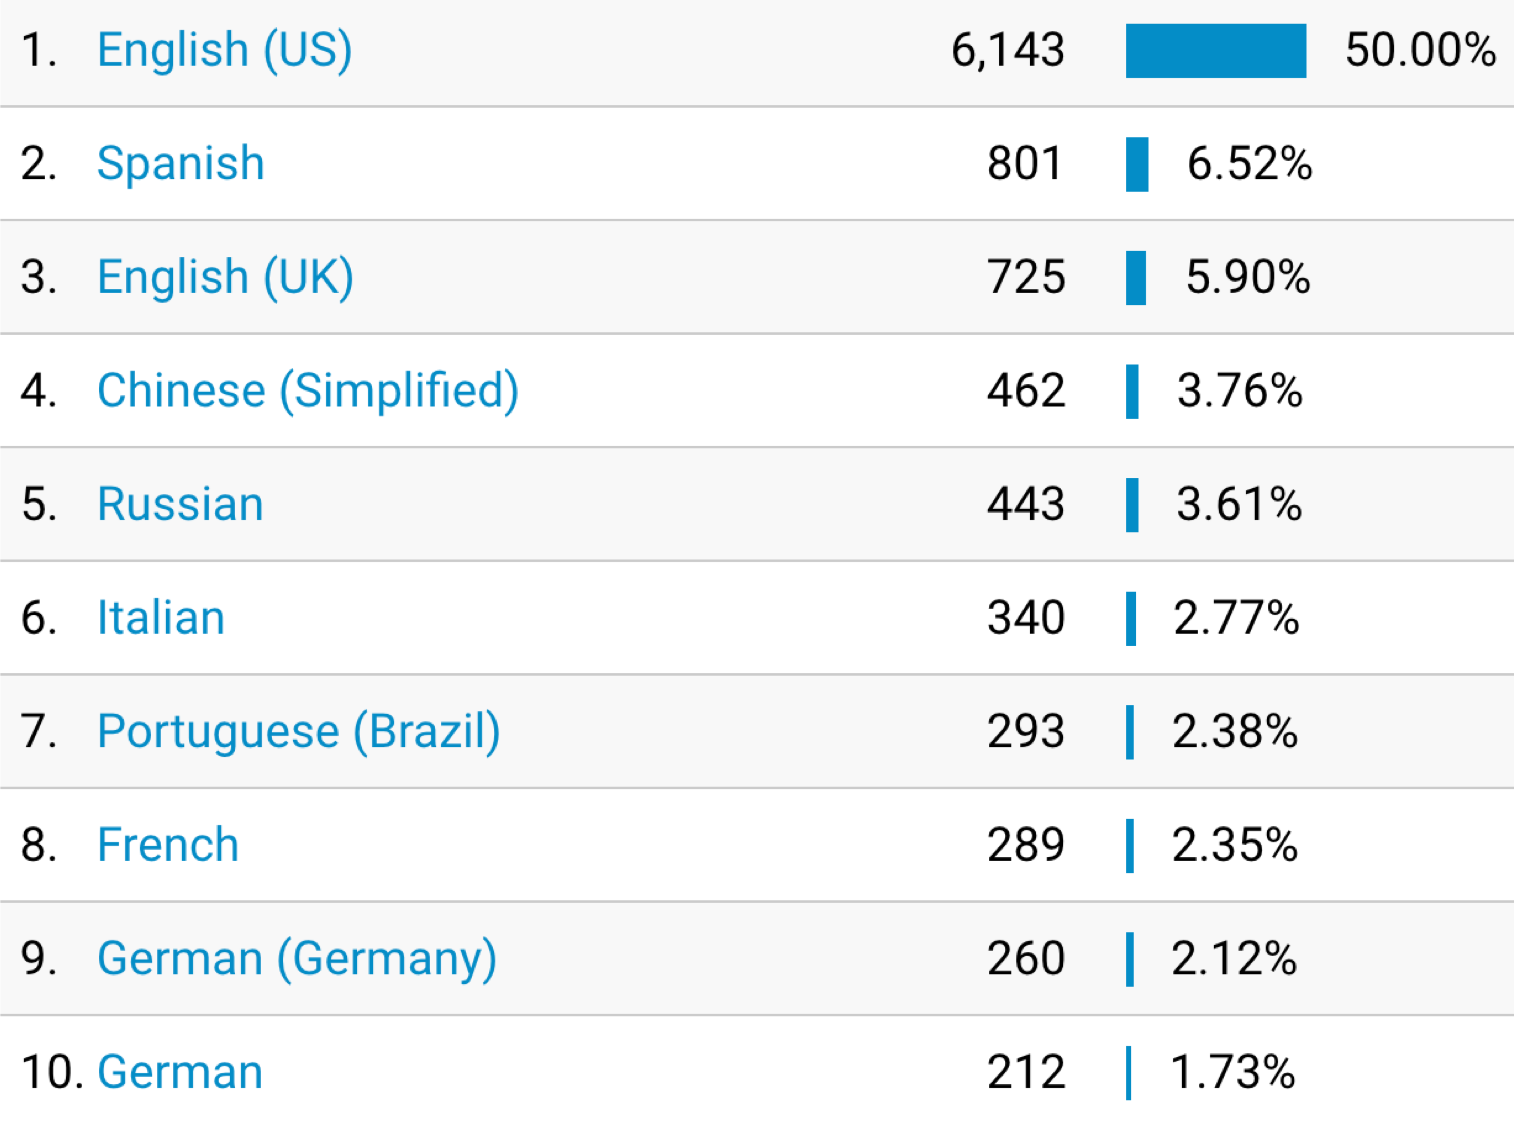
\includegraphics[width=1.0\textwidth]{figuresS/user_languages.png}
	\caption{Languages that HabitLab users set as their preferred language to show webpages in. English is the preferred language of half of our users. \msb{the figures in this sectin of the document are all really large, take up whole page, I suggest scaling down}}
\label{fig:user_languages}
\end{figure}

The users were not explicitly recruited, but were rather all organic installs who discovered the extension/app via sources such as the Chrome/Play store, or were referred to it via press coverage in sources such as Wired or the New York Times.

% Users discover the extension through news articles (it has been mentioned in Wired and the New York Times), the Chrome store, or links from an unrelated open-source project by the author.

Users are asked to read and provide consent to the research protocol upon installation. They may opt out of data collection if they do not wish to have their data analyzed for research purposes.

\section{Design principles and tradeoffs}

We designed HabitLab from the start intending it to be a in-the-wild experimentation platform with a large number of users who would voluntarily and organically install it. As a result, we made a number of design decisions that prioritize growth and retention.

Interventions can all be disabled by the end user, either temporarily for the duration of a session via a ``Turn off'' \msb{watch out for "word quotes", use ``latex quotes''} \geza{done} button shown on each intervention, or permanently. This is intended to boost retention by preventing uninstalls caused by users disliking a particular intervention. While this complicates some analyses -- for instance, we may have fewer samples about the effectiveness of less popular interventions that tend to be disabled more -- we believe this to be the appropriate tradeoff.

Interventions are designed to be minimally intrusive. While in principle users can just disable interventions they do not like, we still found that many users would uninstall after seeing particular, intrusive interventions. We saw this pattern most notably with interventions that have interstitial screens -- that is, they prevent the user from interacting with the page until they have gone through the intervention. As a result, with the exception of a handful of interventions which must be in the interstitial format -- for instance, forcing the user to wait for 10 seconds before loading the page -- we tried to avoid interstitial interventions as much as possible.

Interventions are designed to load fast, and as a result we ensure that all interventions can work offline and do not depend on remote network resources that might take a long time to load. We found that for interventions that take a second to load or more, the uninstall rate would increase after seeing them. This effect is particularly evident with interstitial interventions, which would have the jarring effect of allowing the user to use the site for a few seconds and disrupting them with an interstitial page once the intervention loads.

We have a simple and short onboarding process. Notably, we do not have long demographic surveys that characterize other similar research projects like LabInTheWild, relying on data from Google Analytics to gather demographic data instead. While data from Google Analytics is only approximate -- it is estimated from browsing patterns rather than from asking users directly -- we believed that if the data is accurate enough to be used by market research companies worldwide, it would be adequate for our purposes. Furthermore, requiring users to complete onboarding demographic surveys would not be able to guarantee that users would answer truthfully.

This principle of minimizing the amount of questions the user must answer also extends beyond the onboarding process. We make only minimal usage of experience sampling. We do so because we saw in one of our studies that even minimally intrusive, single-click experience sampling prompts that users can safely ignore will significantly increase the uninstall rate. As a result, most of the data we are able to gather is quantitative in nature, and we are only able to gather limited qualitative data from what users report to us through email, our feedback pages, reviews left on app store pages, or the uninstall survey.

% shown in Figure \ref{fig:onboarding_nudges}, some ``generic'' interventions can be used on all sites, and others were developed specifically for a particular site such as Facebook or Youtube.

%\begin{figure}
%  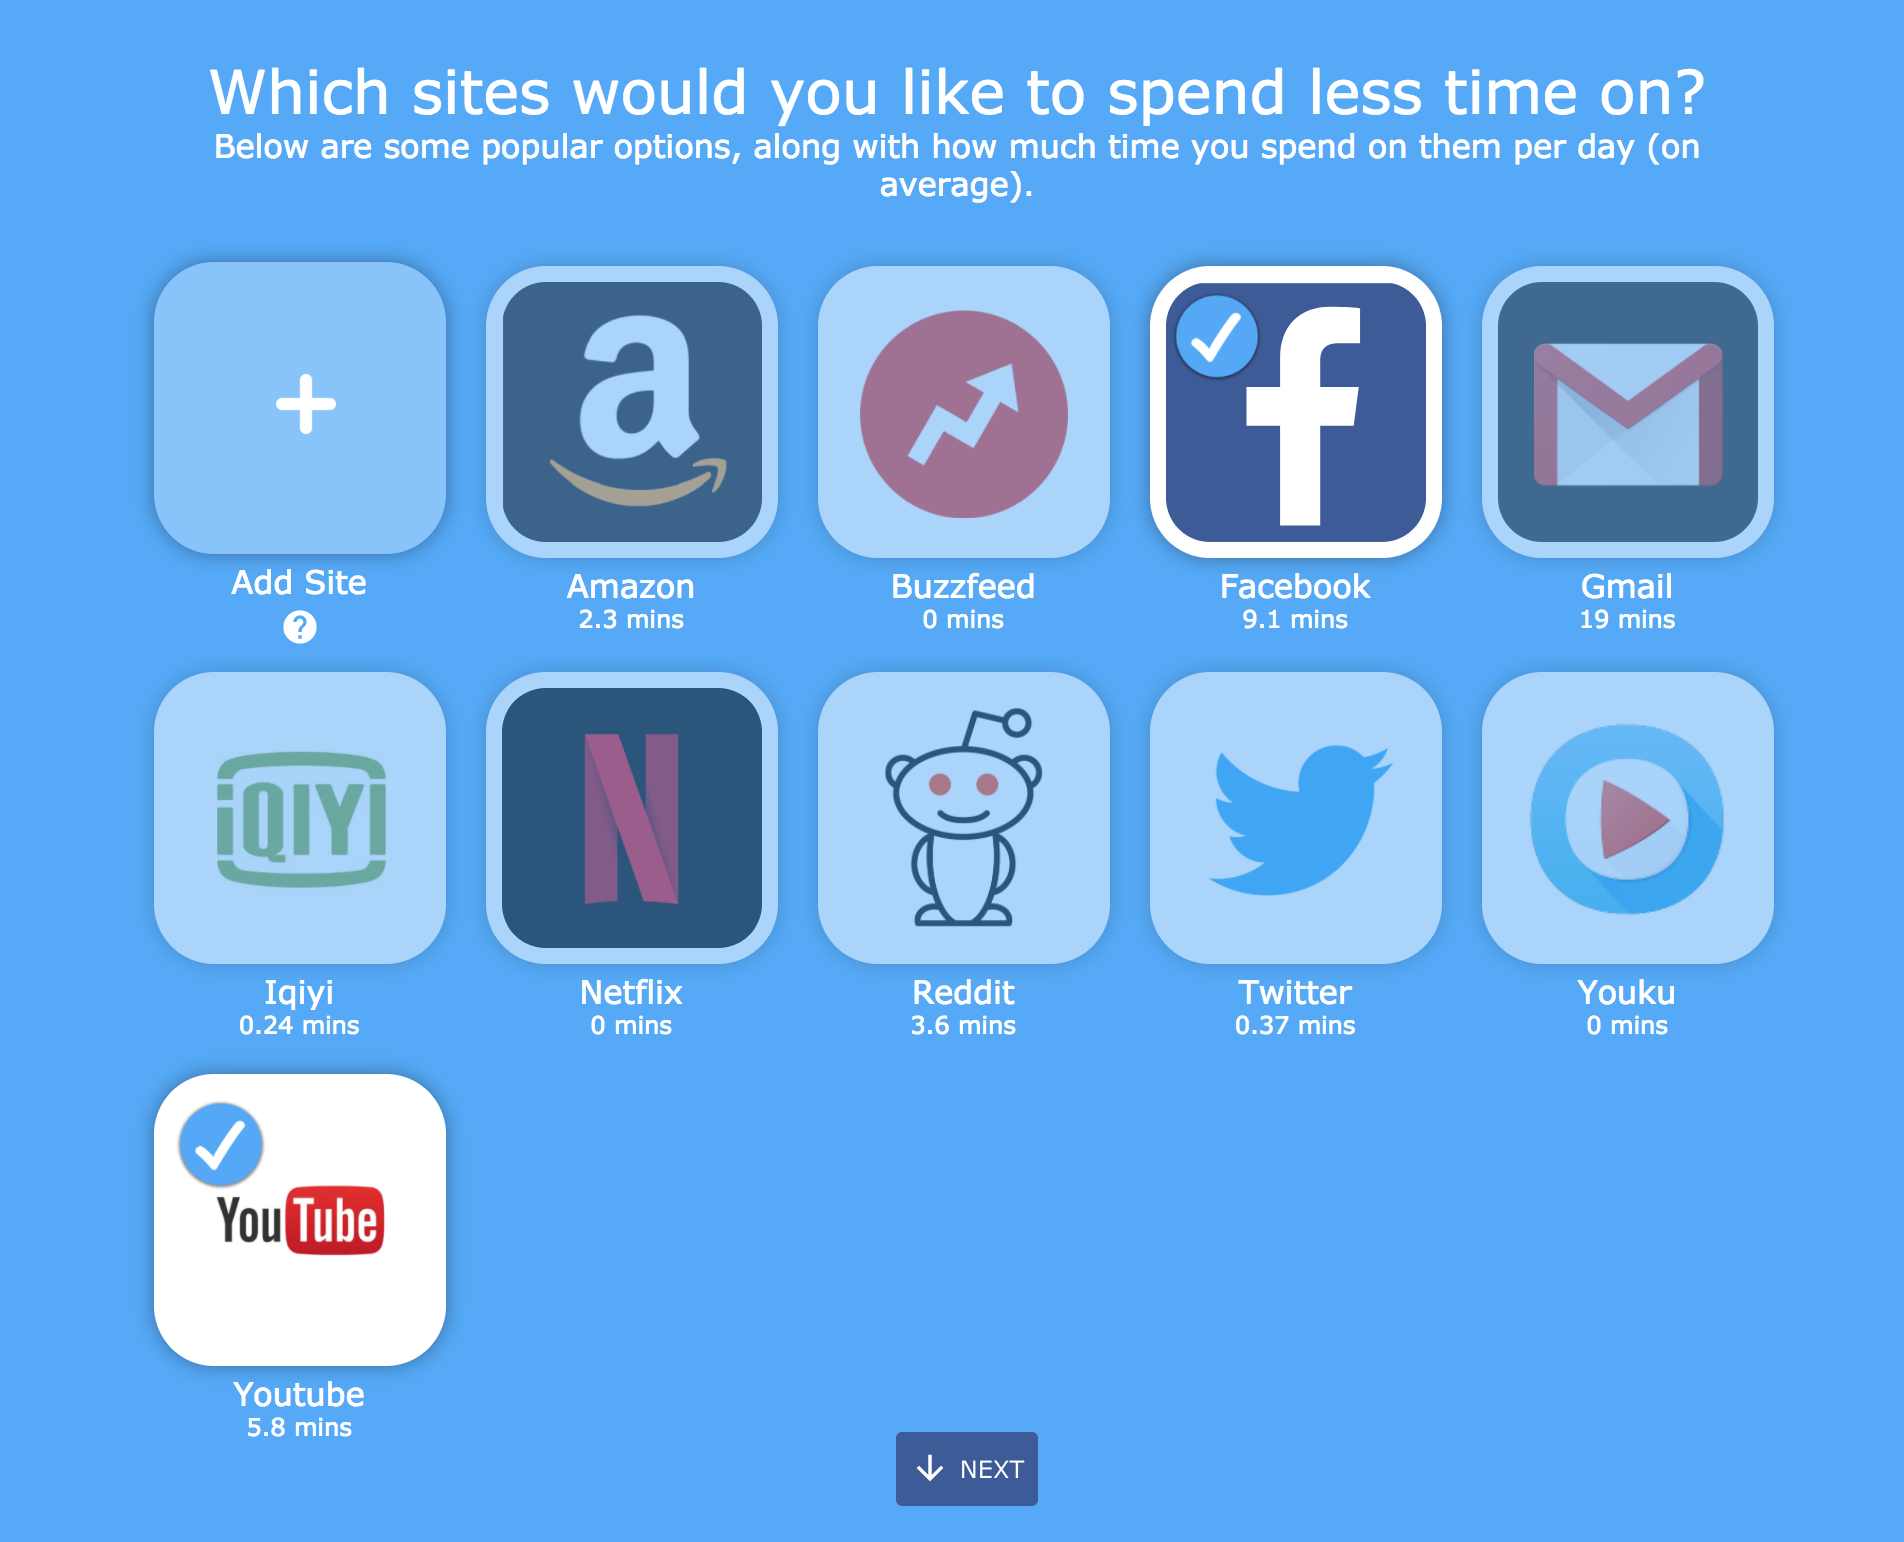
\includegraphics[width=\textwidth]{figures/onboarding_sites}
%  \caption{During onboarding, users first select sites to spend less time on.}
%  \label{fig:onboarding_sites}
%\end{figure}

%\begin{figure}
%  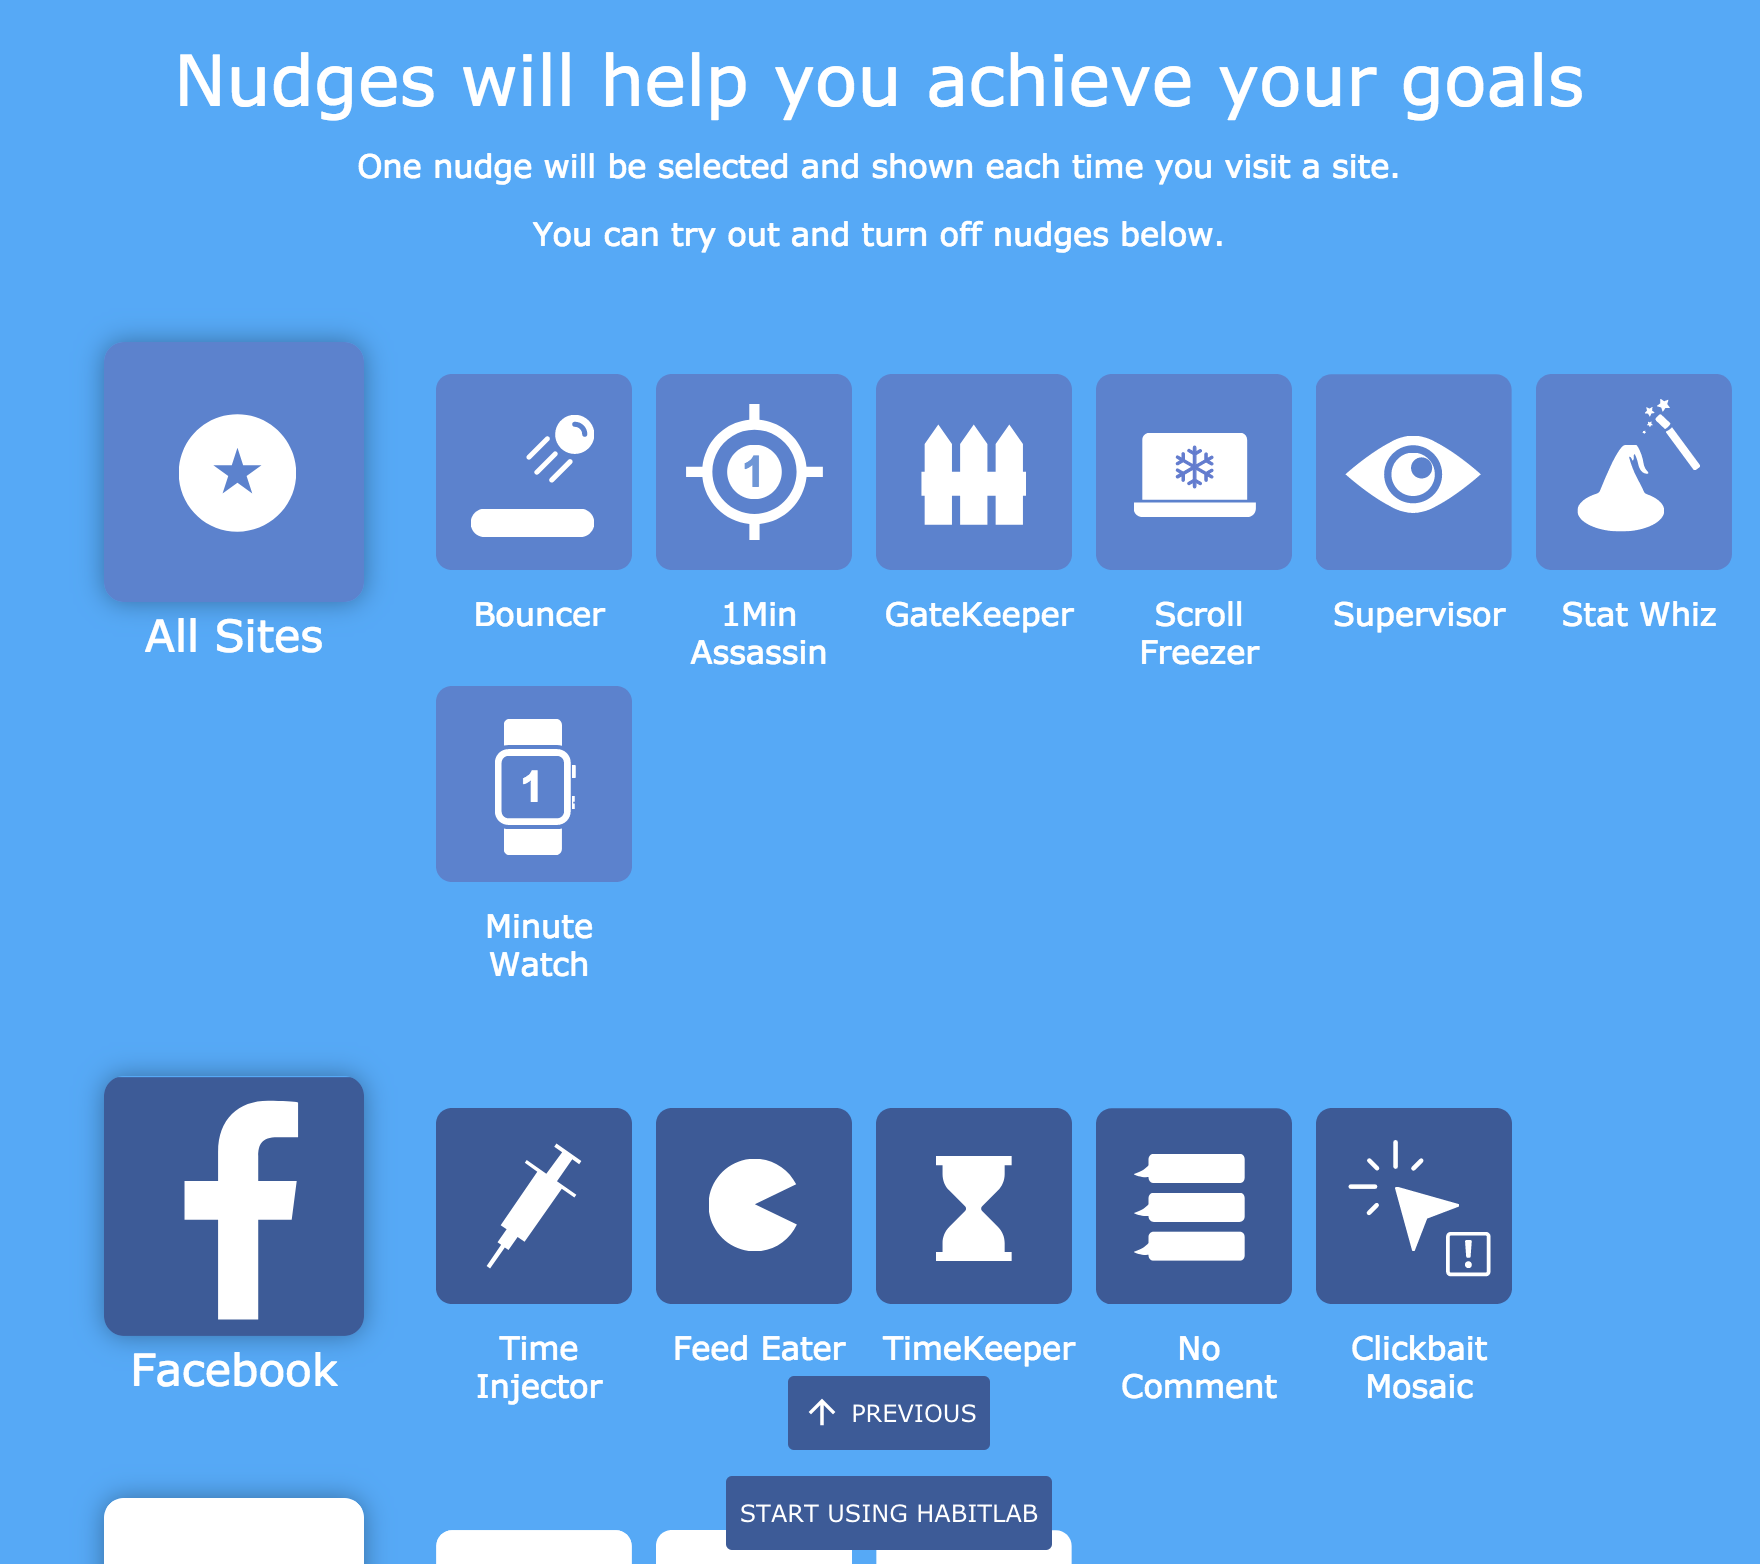
\includegraphics[width=\textwidth]{figures/onboarding_nudges_short}
%  \caption{Users are then presented with the nudges (interventions) they will see on each site.}
%  \label{fig:onboarding_nudges}
%\end{figure}


